% !TeX encoding = UTF-8

%==============================================================================
% Modelo de Dissertação para Trabalho de Conclusão de Curso Ciência da Computação
% do Centro Universitário Dinâmica das Cataratas de Foz do Iguaçu
% Autor: Miguel Diogenes Matrakas, Thiago Medeiros de Souza
% 2016/2017
% ----
%
% ADAPTADO DE:
% Modelo de Tese/Dissertação
% Autora: Fabiana Frata Furlan Peres 
% 2014 
% ----
%
% ADAPTADO DE:
% modelo de Documento TCC da Unioeste   
% que por sua vez foi ADAPTADO DE: 
% abtex2-modelo-trabalho-academico.tex, v-1.6 laurocesar
% Copyright 2012-2013 by abnTeX2 group at http://abntex2.googlecode.com/ 
% ---
% abnTeX2: Modelo de Trabalho Academico (tese de doutorado, dissertacao de
% mestrado e trabalhos monograficos em geral) em conformidade com 
% ABNT NBR 14724:2011: 
% Informacao e documentacao - Trabalhos academicos - Apresentacao
%==============================================================================

%==============================================================================
% DECLARAÇÃO DO TIPO DE DOCUMENTO, TAMANHO DA FOLHA E FONTE
%==============================================================================
\documentclass[12pt,oneside,a4paper,english,brazil]{cc-udc-abntex2}


%==============================================================================
% DEFINIÇÃO DOS PACOTES UTILIZADOS
%==============================================================================
\usepackage{cmap}		% Mapear caracteres especiais no PDF
%\usepackage{lmodern}	% Usa a fonte Latin Modern			
%\usepackage{uarial}		% Usa a fonte uarial - um clone livre da fonte arial (arial é uma fonte comercial, protegida)
%\usepackage{helvet}
\usepackage[T1]{fontenc}% Selecao de codigos de fonte.
\usepackage[utf8]{inputenc}	% Codificacao do documento (conversão automática dos acentos)
\usepackage{indentfirst}% Indenta o primeiro parágrafo de cada seção.
%\usepackage{color}		% Controle das cores
\usepackage{graphicx}	% Inclusão de gráficos
\usepackage{amsmath}	% Definições da Sociedade Americana de Matemática
\usepackage{amssymb}	% Definições da Sociedade Americana de Matemática
\usepackage{amsthm}		% Definições da Sociedade Americana de Matemática
\usepackage{hyphenat}	% comandos para separação silábica
\usepackage[alf,abnt-emphasize=bf,bibjustif]{abntex2cite} % Citações padrão ABNT
%\usepackage{pifont}		% Fonte de simbolos matemáticos
%\usepackage{latexsym}	% Fonte de simbolos
%\usepackage{url}		% Formatação de URLs - quebra de linha nas referências
%\usepackage{multirow}	% Celulas de tabela que ocupam multiplas linhas
%\usepackage{longtable}	% Tabelas longas, em mais de uma página
%\usepackage{marginnote} % Anotações nas margens do documento
%\usepackage[listofformat=subparens,subrefformat=parens,labelformat=parens]{subfig}		% utilização de subfiguras
%==============================================================================
% Pacotes de desenho - criar gráficos, plotar equações, anotar figuras, etc
\usepackage{tikz}		% Ferramenta principal
\usepackage{pgfplots}	% Desenhar gráficos no latex
\usetikzlibrary{positioning}
\usetikzlibrary{calc}
\usetikzlibrary{arrows,shapes,backgrounds}
\pgfplotsset{compat=newest}
%==============================================================================

%==============================================================================
% Caminhos para os diretório com as Imagens
%==============================================================================
\graphicspath{{./Imagens/}{./Graficos/}}

%==============================================================================
% Informações a respeito do trabalho
%==============================================================================
% ---
% INFORMAÇÕES REFERENTE A DISSERTAÇÃO
% ---

\titulo{UTILIZAÇÃO DE REDES NEURAIS ARTIFICIAIS PARA A PREDIÇÃO EM BOLSAS DE VALORES ATRAVÉS DE SÉRIES TEMPORAIS}
\autor{Fernando Demarchi Natividade Luiz}
\autorcitado{Luiz, Fernando Demarchi Natividade}
%\segundoautor{Tarcisio Matheus Saraiva da Cruz}
%\segundoautorcitado{CRUZ, Tarcisio Matheus Saraiva}
\orientador{Prof. Me. Valmei Abreu Júnior}
\coorientador{Prof. Dr. Miguel Diógenes Matrakas}
\data{2017}
\codigoautor{A000} % solicitar o código ao bibliotecário da instituição
\codigopublicacao{CDD: 123.432 }  % solicitar o código ao bibliotecário da instituição - Também pode ser padrão -> CDU: 02:141:005.7
\palavrachaveum{Palavra-chave 1}
\palavrachavedois{Palavra-chave 2}
\palavrachavetres{Palavra-chave 3}
 % DADOS para CAPA e FOLHA DE ROSTO


%==============================================================================
% CONFIGURAÇÕES DA APARENCIA DO PDF FINAL
%==============================================================================
\makeatletter
\hypersetup{     	
	pdftitle={\@title}, 
	pdfauthor={\@author},
	pdfsubject={\imprimirpreambulo},
	pdfcreator={LaTeX with abnTeX2},
	pdfkeywords={}{}{}{}, 
	colorlinks=true,       		% false: boxed links; true: colored links
	linkcolor=black,          	% color of internal links
	citecolor=black,        	% color of links to bibliography
	filecolor=black,      		% color of file links
	urlcolor=black,
	bookmarksdepth=3
}
\makeatother


%==============================================================================
% Constroi o índice remissivo
%==============================================================================
\makeindex


%==============================================================================
% SEPARAÇÃO DE SILABAS
% Incluir palavras que o LaTeX não realizar a separação silábica corretamente no texto
%==============================================================================
%\hyphenation{}
\hyphenation{Mar-ca-ção}
\hyphenation{lin-gua-gem}
\hyphenation{pro-fis-sio-nais}
\hyphenation{ar-qui-vos}
\hyphenation{fer-ra-men-tas}
\hyphenation{ma-te-ri-al}

%==============================================================================
% INÍCIO DO DOCUMENTO
%==============================================================================
\begin{document}
\frenchspacing % Retira espaço extra obsoleto entre as frases.

%==============================================================================
% ELEMENTOS PRÉ-TEXTUAIS
%==============================================================================
\imprimircapa
\imprimirfolhaderosto* % (o * indica que haverá a ficha bibliográfica)

%\input{Configuracoes/ficha_catalografica}
%\imprimirfichacatalografica
%% ---
% FOLHA DE APROVAÇÃO
% ---
\begin{folhadeaprovacao}
\begin{center}
	\vspace*{1cm}  
  	\large\textbf{TERMO DE APROVAÇÃO}
  	
  	\vspace*{1cm}
  	%\vspace*{2cm}
  	{\large\textbf\imprimirautor}

   \vspace*{1cm}
   %\vspace*{2cm}
    {\large\textbf\imprimirtitulo}   
 \end{center}     
  
	
	\hspace{.4\textwidth}
	\SingleSpace\noindent\normalsize{Trabalho de conclusão de curso apresentado como requisito obrigatório para obtenção do título de Bacharel em Ciência da Computação da Faculdade Anglo-Americano de Foz do Iguaçu, pela seguinte banca examinadora:}
%	\noindent\paragraphq
   
 %  \end{center}
    
   %\vspace*{1.5cm}
   \vspace*{0.5cm}  %minha modif
   \assinatura{{\imprimirorientador}\\{\small \imprimirinstituicao\\(Orientador)}}
   \assinatura{Prof. Banca 2\\{\small\imprimirinstituicao}}
   \assinatura{Prof. Banca 3\\{\small\imprimirinstituicao}}
   \vspace*{2.5cm}
   \begin{center}
   	{\imprimirlocal, \ \imprimirdata}
   	%{Foz do Iguaçu, 12 de junho de 2016}
   \end{center}
   
 
\end{folhadeaprovacao}
%% ---
% DEDICATÓRIA
% ---
\begin{dedicatoria}
   \vspace*{\fill}
   \begin{flushright}
   	\textit{Dedico este trabalho a meus pais, \\ Sr... e Sra... \\ que, com muito amor, me ensinaram os valores da vida.}
   	
   \end{flushright}
\end{dedicatoria}

%% ---
% AGRADECIMENTOS
% ---
\begin{agradecimentos}[AGRADECIMENTOS]
Primeiramente agradeço a Deus por sua graça e salvação.

À minha família, por terem me proporcionado ...

À ... por me mostrar o caminho da ...

Aos meus grandes amigos....

A todos os professores que fizeram parte desta importante etapa da minha vida.

Aos meus orientadores.....


\end{agradecimentos}


%% ---
% EPÍGRAFE
% ---
\begin{epigrafe}
    \vspace*{\fill}
	\begin{flushright}
		\textit{
		``Once you have eliminated the impossible, whatever remains,\\
		 however improbable, must be the truth.''\\
		\-- Mr. Spock, Star Trek (2009)	
		}
	\end{flushright}
\end{epigrafe}


%\vspace*{-0.65cm}
%% ---
% RESUMO PORTUGUÊS
% ---
\begin{resumo}[RESUMO]	
A predição no mercado eletrônico financeiro é um desafio considerável para proporcionar aos investidores uma boa capacidade de atuação no processo de compra e venda de ações. Tendo isso em vista, técnicas computacionais vêm sendo aplicadas arduamente para realizar análises dentro deste cenário de atuação. Dentre as técnicas, as Redes Neurais Artificiais (RNAs), uma subárea da Inteligência Artificial, que busca simular computacionalmente a forma de processamento do cerébro humano, vem ganhando destaque para este propósito. Sendo assim, este trabalho apresenta a especificação e aplicabilidade de um modelo de RNA para realizar predições no valor de abertura das ações na bolsa de valores NASDAQ. Além disso, são evidenciadas e detalhadas ferramentas que auxiliam o desenvolvimento dessa técnica de forma eficiente, utilizando a linguagem de programação Python e suas bibliotecas para análise de dados.

\vspace{\onelineskip}
    
\noindent
\textbf{Palavras-chaves}: Redes Neurais Artificiais. Inteligência Artificial. Mercado Financeiro. Python.
 % 4 palavras separadas por . (ponto)
\end{resumo}

%\vspace*{-0.65cm}
%% ---
% RESUMO INGLÊS
% ---
\begin{resumo}[ABSTRACT]
 \begin{otherlanguage*}{english}
The social network ....

   
   \vspace{\onelineskip}
 
   \noindent 
   \textbf{Keywords}: Data. Data Mining. Twitter. Python.
 \end{otherlanguage*}
\end{resumo}


\pdfbookmark[0]{\listfigurename}{lof}		% inserir lista de ilustrações
\listoffigures*
\cleardoublepage

%\pdfbookmark[0]{\listtablename}{lot}			% inserir lista de tabelas
%\listoftables*
%\cleardoublepage

\pdfbookmark[0]{\lstlistlistingname}{lol}	% inserir lista de códigos
\counterwithout{lstlisting}{chapter}
\begin{KeepFromToc}
\lstlistoflistings
\end{KeepFromToc}
\cleardoublepage

\pdfbookmark[0]{\listofgraficosname}{logr}	% inserir lista de gráficos
\listofgraficos*
\cleardoublepage

% ---
% SIGLAS
% ---
\begin{siglas}
	\item[API] \textit{Application Programming Interface} - Interface de programação de aplicações
	\item[BSD] \textit{Berkeley Software Distribution}
	\item[EAM] Erro Absoluto Médio
	\item[EQM] Erro quadrático médio
	\item[IDE] \textit{Integrated Development Environment} - Ambiente de Desenvolvimento Integrado
	\item[MACD] \textit{Moving Average Convergence Divergence} - Convergência e Divergência de Médias Móveis
	\item[MLP] \textit{Multilayer Perceptron} - Perceptron de Múltiplas Camadas
	\item[NASDAQ] \textit{National Association of Securities Dealers Automated Quotation System}
	\item[PyBrain] \textit{Python-Based Reinforcement Learning, Artificial Intelligence and Neural Network Library} - Reforço de aprendizagem baseada em Python, Biblioteca de Inteligência Artificial e Rede Neural
	\item[REQM] Raiz do Erro Quadrático Médio
	\item[SQL] \textit{Structured Query Language} - Linguagem de Consulta Estruturada
	\item[SVM] \textit{Support-Vector-Machines } - Máquinas de Vetores de Suporte 
\end{siglas}

  				% inserir lista de abreviaturas e siglas

%\begin{simbolos}
  \item[$ \Gamma $] Letra grega Gama
  \item[$ \Lambda $] Lambda
  \item[$ \zeta $] Letra grega minúscula zeta
  \item[$ \in $] Pertence
\end{simbolos}
				% inserir lista de símbolos

\vspace*{0cm}
\pdfbookmark[0]{\contentsname}{toc}			% inserir o sumario
\tableofcontents*
\cleardoublepage


%==============================================================================
% ELEMENTOS TEXTUAIS
%==============================================================================
\textual
\pagestyle{abnt_CC-UDC}

%!TeX encoding = UTF-8

\chapter{INTRODUÇÃO}\label{ch:introducao}

A informatização do mercado acionário, que permite a movimentação de compra e venda de ações de forma eletrônica e automática, tornou-se fundamental ao longo das últimas décadas, gerando uma série de mudanças na forma em que as negociações são realizadas, se comparado ao modelo de negociação anterior, onde as movimentações aconteciam em uma unidade central, com a presença física dos investidores. Portanto, esse novo modelo mudou a forma de atuação nas bolsas de valores, possibilitando a movimentação de capitais \textit{online}, facilitando e aumentando a gama de possibilidades para a aquisição de novos acionistas. Atualmente, os papéis negociados mais relevantes em bolsas de valores, vêm de grandes empresas que dominam o mercado em suas respectivas áreas, gerando uma alta movimentação financeira que pode conceber um impacto tanto positivo como negativo no setor econômico, influenciando em decisões políticas e sociais que afetam não só a esfera econômica, mas também todos os níveis da sociedade \cite{shiller}.

Em contrapartida, houve, automaticamente, um impacto computacional significativo sobre esse novo paradigma do mercado de ações. Com o advento da Internet e o fácil acesso aos dados históricos dos papéis negociados nas bolsas de valores, através de     \textit{sites} que disponibilizam essas informações, técnicas computacionais têm se tornado uma grande aliada para o diagnóstico dos preços de ações e índices, aumentando significamente as pesquisas e os modelos computacionais que possam auxiliar no aperfeiçoamento e análise do mercado financeiro.

A complexidade em prever valores futuros no mercado de ações, é um estímulo consideravelmente grande para a comunidade científica internacional, tendo em vista a diminuição do risco de investimento em ativos financeiros. Nesse contexto, técnicas como aprendizado de máquina, Redes Neurais Artificiais  e outras soluções de inteligência artificial, vêm sendo aplicadas arduamente para possibilitar um aumento significativo na predição de valores no mercado acionário \cite{gambogi}.

Dessa maneira, uma abordagem que vem ganhando destaque, dentre as pesquisas referentes à predição de cotações futuras que utilizam séries temporais, são as Redes Neurais Artificiais (RNAs). A capacidade das RNAs em trabalhar com uma quantidade significativa de variáveis simultâneas, além da composição de sua estrutura maciçamente paralela e distribuída, evidenciam sua alta escala de poder computacional, concedendo-as habilidades de aprendizado e generalização de funções. Estas duas capacidades de processamento de informação, tornam possíveis para as RNAs resolver problemas de grande escala que, usando o processamento digital convencional, são consideradas computacionalmente inviáveis e intratáveis \cite{elpink, haykin2000}.

Neste sentido, dada a importância das RNAs na predição de cotações futuras de ações em bolsas de valores, o presente trabalho apresenta um estudo da aplicação destas RNAs na previsão de preços futuros dos mais relevantes papéis da NASDAQ \textit{Stock Market}, o segundo maior mercado de ações do mundo, palco onde as maiores empresas de tecnologias investem e controlam seus ativos financeiros.


\section{JUSTIFICATIVA}\label{sec:justificativa}

São vários os aspectos que nos levam a tentar realizar a previsão de índices acionários no mercado de investimentos. De fato, faz-se o principal motivo, garantir maior lucratividade possível com a realização de bons investimento, fazendo com que os investidores obtenham sempre uma vantagem sobre os demais que atuam no mercado financeiro.

Outro fator motivacional para a realização desta predição, utilizando RNAs, se dá pela sua capacidade de adaptação a mudanças bruscas e repentinas nos dados a serem analisados, sem que se afete a acuracidade de seus resultados, por não se tratar de um modelo pré-definido \cite{marangoni}.

O crescimento da utilização de RNAs aplicadas a importantes áreas do contexto social, é mais um fator motivacional para sua utilização. Além da aplicação na área financeira apresentada neste trabalho, ferramentas tecnológicas que implementam esta inteligência computacional têm-se feito úteis em áreas como: recursos humanos, marketing, medicina, engenharia, dentre outras. Na área da medicina, por exemplo, é válido citar sua utilidade no diagnóstico e, até mesmo, na prevenção de futuras doenças e patologias \cite{marangoni}.

Portanto, a variação dos preços das ações proporcionada por oscilações diárias, é uma excelente diretriz para o aperfeiçoamento de análises referente à inteligência computacional, dispondo de um ambiente propício para a aplicabilidade sobre séries temporais, através do acesso a uma quantidade contínua de dados que viabiliza criar e aprimorar diversos padrões de RNAs \cite{gambogi}.



\section{OBJETIVOS}\label{sec:objetivos}
A partir do tema definido, estabelecem-se os objetivos a serem alcançados ao término deste trabalho. Assim temos, respectivamente, o objetivo principal e os objetivos específicos, apresentados em ordem lógica de desenvolvimento.
\subsection{Objetivo Geral} 
Atribuiu-se, como objetivo principal deste trabalho, especificar e aplicar um modelo de RNA para análise e predição de valores acionários através de séries temporais.

\subsection{Objetivos Específicos}\label{subsec:objetivos_especificos}
Com o objetivo geral determinado, tornaram-se necessários as definições de alguns objetivos específicos, sendo:
\begin{itemize}
	\item Especificar uma arquitetura de RNA;
	\item Definir um ambiente para o desenvolvimento da RNA;
	\item Utilizar uma Interface de programação de aplicações (API) para a coleta dos dados que serão analisados;
	\item Treinar o modelo de RNA especificado;
	\item Realizar testes com o modelo treinado, através das ações utilizadas;
	\item Analisar os resultados obtidos pela implementação, comparando-os com os seus resultados reais e avaliando sua capacidade de precisão.
\end{itemize}

\section{ESTRUTURA DO DOCUMENTO}\label{sec:organizacao-trabalho}
Este documento será organizado em sete capítulos: introdução, revisão bibliográfica, fundamentação teórica, materiais e métodos, implementação, resultados, conclusões e referências bibliográficas.

O presente capítulo contextualiza e introduz o assunto a ser tratado, bem como define os objetivos a serem alcançados.

No segundo capítulo, são apresentados os trabalhos que foram utilizados como referência e motivação, além de demonstrar suas contribuições científicas.

A fundamentação teórica apresentada no terceiro capítulo, descreve o embasamento referente aos conceitos das técnicas que serão utilizadas para a realização deste estudo.

O quarto capítulo é destinado ao detalhamento de métodos, técnicas e procedimentos que têm por objetivo gerar conhecimento para viabilizar um melhor ambiente de desenvolvimento para o trabalho.

O quinto capítulo detalha a implementação dos métodos, que segue as especificações das técnicas levantadas no capítulo anterior.

No sexto capítulo são expostos os experimentos realizados sobre o protótipo implementado, dispondo os resultados em situações como análise da eficácia de predição e comparação a modelos distintos.

Por fim, no sétimo capítulo são tratadas as conclusões obtidas pela técnica de RNA desenvolvida, destacando suas vantagens e desvantagens. Também serão idealizadas alternativas para trabalhos futuros, os quais dariam continuidade e complementariam a pesquisa realizada.

%==============================================================================
% CAPÍTULOS DA DISSERTAÇÃO
%==============================================================================
% !TeX encoding = UTF-8

\chapter{REVISÃO BIBLIOGRÁFICA}\label{ch:rev-bibs}

Várias técnicas conjugadas à inteligência artificial foram desenvolvidas e vêm sendo aperfeiçoadas ao longo do tempo, com o objetivo de possibilitar predições de boa acuracidade, tal como o estudo realizado por \citeonline{clements} que trabalharam com predições utilizando regressão linear. Dentro dessa linha, também estão presentes as pesquisas que se basearam na utilização de RNAs, que são citadas como referência para analisar a oscilação do mercado acionário, como os estudos realizados por \citeonline{faria}, \citeonline{kara} e \citeonline{white}, além de trabalhos desenvolvidos utilizando algoritmos genéticos, como apresentado no trabalho de \citeonline{nayak}.

O primeiro modelo para previsão de preços no mercado de ações baseado em RNA, foi desenvolvido por \citeonline{white}, o autor utilizou um padrão de rede recorrente, denominado Feedforward, com o objetivo de analisar os retornos diários das ações da International Business Machines (IBM), para testar a teoria do mercado eficiente, proposta por \citeonline{fama}, retratando que a oscilação dos preços das ações seguem uma tendência aleatória. Com bons resultados obtidos através da implementação da RNA, desde então, foi potencializada a quantidade de pesquisas referente à técnica utilizada.

Um dos trabalhos pioneiros em predição no mercado acionário com o auxílio de RNAs, foi o proposto por \citeonline{kamijo}, que utilizaram RNAs recorrentes para o reconhecimento de padrões, através dos gráficos gerados pela análise técnica da bolsa de Tóquio. O objetivo da pesquisa foi encontrar padrões classificados como possíveis indicadores de tendências para o investimento em um determinado ativo.  

Trabalhos posteriores, como o realizado por \citeonline{ding}, define a não existência de um paradigma adequado para predições com o uso de RNAs, necessitando da análise e identificação do problema para especificar o melhor modelo de arquitetura a ser aplicado. \citeonline{ding} também evidenciam a complexidade em especificar parâmetros relevantes para a fase de treinamento de uma RNA, pois o mesmo impacta diretamente no resultado obtido, tornando-se uma etapa de grande relevância na construção de um modelo estável.

Em seu estudo \citeonline{guresen} descreveram a utilização das RNAs como uma das melhores técnicas para modelar o mercado de ações, porque as mesmas podem ser facilmente adaptadas às mudanças do mercado acionário. Em seu trabalho, os autores utilizam uma rede Multilayer Perceptron (MLP) com um total de 80 neurônios, utilizando 20 para a camada de entrada, 40 para a camada oculta, e 20 para a camada de saída, aplicando o algoritmo Backpropagation como forma de treinamento, empregada para prever os valores dos índices das bolsas de valores americanas.

A utilização de RNAs em séries temporais, tem como referência o trabalho realizado por \citeonline{waibel} que evidencia duas abordagens para análise de séries temporais: Dimensionamento temporal e RNAs recorrentes. Em sua pesquisa, foi abordada a capacidade de generalização da RNA sobre um ambiente desconhecido, podendo auxiliar na resolução dos problemas que contam com diversos padrões distintos e com alta complexidade computacional. \citeonline{waibel} utilizou uma rede Feedforward para testar predições que obtivessem resultados relevantes e satisfatórios, utilizando um padrão de previsão denominado One Step Ahead. Este padrão trabalha, segundo o autor, com uma distribuição de  N variáveis de entradas, através de uma alimentação iterativa até o momento T, onde a unidade de saída é representada por T + 1.

\citeonline{zhang} também destacam modelos de previsões através de RNAs. O trabalho enfatizou a realização de múltiplas previsões futuras, denominado Multiple Step Ahead. Os autores descrevem dois métodos apresentados na literatura para  este padrão, previsão iterativa e método direto. No primeiro método, os  valores de predição são usados iterativamente, como material para previsões futuras. Neste caso, apenas um neurônio de saída é necessário. O segundo método, consiste em colocar várias saídas na RNA, correspondente ao resultado esperado da previsão, tendo maior  relevância e utilidade  para ambientes específicos e controlados.

Trabalhos recentes utilizando métodos híbridos também vêm sendo dedicados para melhorar a capacidade de modelagem sobre séries temporais. Na pesquisa produzida por \citeonline{khandelwal} foi utilizado uma abordagem que cruza características do modelo matemático ARIMA com o de uma RNA. Os autores testaram os métodos ARIMA e RNA para separar componentes lineares e não-lineares, respectivamente, de séries temporais em valores econômicos, com o objetivo de encontrar um melhor padrão para tratar a oscilação dos dados obtidos.

Outra abordagem híbrida conhecida na literatura por ter resultados significativos juntamente com as RNAs, são os Mapas Cognitivos Fuzzy (FCMs). No trabalho realizado por \citeonline{lu} por exemplo, é demonstrado o uso de um FCM trabalhando como um modelo de RNA recorrente, capacitando o protótipo a operar através de aprendizado, integrando assim as características de ambas as técnicas aplicadas.

É importante salientar que os trabalhos citados neste capítulo, por alguma peculiaridade ou detalhe técnico serviu como motivação para a idealização deste estudo, não podendo então deixar de citá-los. Além disso, provaram ser referência dentro de suas respectivas problemáticas, trazendo análises e conclusões significativas, que são essenciais para o aperfeiçoamento acadêmico e científico.

Portanto é almejado nos capítulos posteriores, adquirir conhecimento teórico suficiente que possibilite a realização de um trabalho que  traga uma contribuição científica relevante, e que sirva como referência para os estudos futuros, como os aqui citados.
% !TeX encoding = UTF-8

\chapter{FUNDAMENTAÇÃO TEÓRICA}\label{ch:fundaments-teorico}
Nos tópicos que seguem, serão apresentados conceitos teóricos sobre o tema proposto, ou seja, será realizada uma contextualização desde o processo de funcionamento de RNAs até sua aplicabilidade no mercado acionário.

%%
% FUNDAMENTOS
\section{FUNDAMENTOS DE REDES NEURAIS ARTIFICIAIS}\label{sec:fundamentos}
As RNAs procuram simular métodos de aprendizado do cérebro humano, através do uso de neurônios interligados. Uma RNA é inspirada nos neurônios biológicos e nos sistemas nervosos, logo, para entender o funcionamento da mesma, é necessário, primeiramente, entender o funcionamento dos neurônios biológicos \cite{neto}.

A partir deste conceito, uma RNA pode ser definida como uma estrutura interligada complexa de processamento, composta por neurônios e conexões \cite{ferreira}.

\subsection{Neurônios Biológicos} 
Os neurônios são células, que desempenham o papel de conduzir os impulsos nervosos. Estas células especializadas são, portanto, as unidades básicas do sistema que processa as informações e estímulos de um cérebro\cite{lent}. 

A Figura 1 representa a estrutura básica de um neurônio biológico. Conceituando os componentes do neurônio, os dendritos são responsáveis pela recepção das informações, possuindo as extremidades ramificadas. O corpo celular é responsável pela integração das informações e os axônios são responsáveis pelo transporte dos impulsos nervosos de um neurônio para outro ou de um neurônio para uma glândula ou fibra muscular \cite{lent}.

\begin{figure}[h]
	\centering
	\fbox{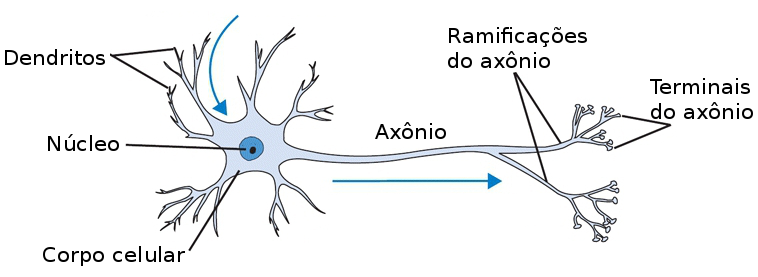
\includegraphics[width=0.6\textwidth]{cerebro}}
	\caption{Representação de um neurônio biológico}
	\fonte{Adaptado de \citeonline{stanford} }
	\label{exec-linearmente-separavel}
\end{figure} 

Cada dendrito possui em torno de mil a dez mil ramificações em suas extremidades. A transmissão de impulsos nervosos por meio da comunicação dos axônios com os dendritos de neurônios adjacentes é chamada de sinapse, por sua vez, tal conjunto forma o sistema nervoso \cite{neto}.

\subsection{Neurônios Artificiais}
A estrutura de um neurônio artificial segue os mesmos conceitos relacionados aos neurônios biológicos, buscando realizar as mesmas funções, utilizando-se de conceitos matemáticos, aritméticos e de tecnologias computacionais.

A Figura 2 esboça a estrutura que compõe um neurônio artificial não-linear, demarcando cada item que o compõe. 

\begin{figure}[h]
	\centering
	\fbox{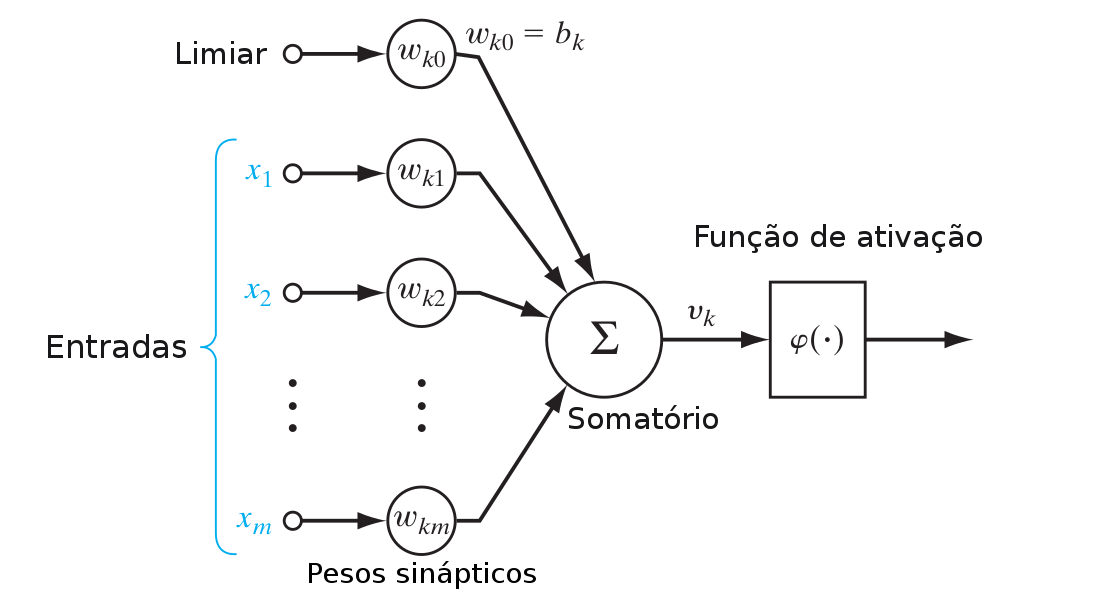
\includegraphics[width=0.8\textwidth]{neuronio}}
	\caption{Representação de um neurônio artificial}
	\fonte{Adaptado de \citeonline{haykin2009} }
	\label{exec-linearmente-separavel}
\end{figure}

Analisando a figura da esquerda para a direita, pode-se observar que: 

\begin{enumerate}
	\item \textit Os sinais de entrada $x_i$ serão processados pela sinapse $wk_i$, conectadas ao neurônio;
	\item \textit As sinapses ou elos de conexão, com seus respectivos pesos sinápticos que se multiplicarão ao sinal de entrada $\theta_i$. Segundo \citeonline{haykin2000}, ao contrário a uma sinapse do cérebro, o peso sináptico de um neurônio artificial pode estar em um intervalo que inclui tanto valores positivos quanto negativos;
	\item \textit O somatório $\sum$, que resulta na soma dos sinais de entrada $x_i$, ponderados pelas respectivas sinapses do neurônio;
	\item \textit A função de ativação, responsável por delimitar os resultados de saída possíveis a um intervalo finito, recebe como entrada o resultado $v_k$ em $\varphi$(.) para gerar o resultado.
\end{enumerate}

\subsection{Redes Neurais Artificiais}\label{sec:redes-neurais}
Uma RNA pode ser definida como uma ferramenta computacional, produzida e programada para realizar análise de dados, tal como seu comportamento e relações, visando trabalhar com os mesmos conceitos de um sistema nervoso, simulando o comportamento de um conjunto de neurônios biológicos. Por meio de complexos processos de treinamento e aprendizagem, as RNAs visam realizar o reconhecimento de padrões de dados, para que possa prever resultados, através de classificação ou generalização dos dados em questão \cite{haykin2009}.

A representação de uma RNA pode ser visualizada na Figura 3, onde os nodos do grafo representam os neurônios, as arestas representam as conexões e as setas representam a direção do fluxo de sinal.

\begin{figure}[h]
	\centering
	\fbox{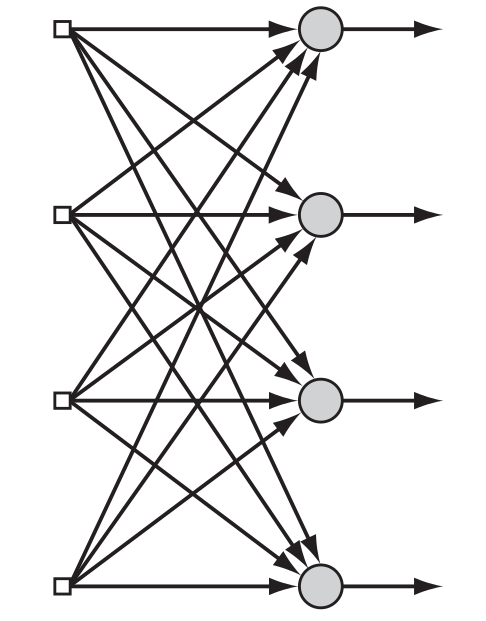
\includegraphics[width=0.5\textwidth, height=0.33\textheight]{RNA}}
	\caption{Representação gráfica de uma Rede Neural Artificial}
	\fonte{\citeonline{haykin2009}}
	\label{exec-rna}
\end{figure}

\section{ARQUITETURA DE REDES NEURAIS ARTIFICIAIS}\label{sec:redes-neurais-arquitetura}
A forma como agrupam-se os neurônios artificiais em uma RNA é uma das principais características que definem seu tipo de arquitetura. Estes agrupamentos são baseados na forma como os neurônios são conectados no cérebro humano, de forma que as informações possam ser processadas dinamicamente ou iterativamente.
 
Biologicamente, as RNAs são organizadas e construídas de forma tridimensional por componentes microscópicos. Há uma forte restrição no número de camadas que a rede pode conter, limitando consideravelmente o tipo e o escopo da implementação da mesma, dependendo da complexidade do problema \cite{haykin2009}.

A arquitetura de uma RNA pode ser classificada pela quantia de camadas ocultas e pelo sentido do fluxo de dados. Em relação ao número de camadas ocultas, ela pode ser de camada única (\textit{single-layer}) ou multicamadas (\textit{multilayer}). Quanto ao sentido do fluxo de dados, ela pode ser alimentada adiante (\textit{feedforward}) ou recorrente (\textit{feedback}) \cite{neto}.

As redes que possuem uma única camada são as que possuem um nó entre sua entrada e saída. Este tipo de rede é indicada para a solução de problemas linearmente separáveis. Já as que possuem multicamadas apresentam uma ou mais camadas entre seu início e fim. Essas camadas são chamadas de camadas escondidas (\textit{hidden}, intermediárias ou ocultas).

A topologia de RNA mais popular atualmente é a rede direta com neurônios estáticos (\textit{feedforward}) juntamente com a perceptron de múltiplas camadas (\textit {Multilayer Perceptron}) que utiliza o algoritmo de retropropagação (\textit{backpropagation}) como forma de treinamento \cite{neto}.

\subsection{Redes Alimentadas Adiante com Camada Única}
A organização de uma RNA em camadas adiante pode ser representada de uma maneira simples, onde os neurônios, distribuídos em camadas, recebem sinais de entrada que são projetados sobre os mesmos. Porém, nesta distribuição não ocorre o contrário, ou seja, o fluxo de alimentação ocorre sempre no sentido adiante ou acíclico.
 
Segundo \citeonline{haykin2000}, na estrutura de camada única, a representação dos nós de neurônios responsáveis por receber e processar os sinais de entrada é dada em uma única camada. Para melhor entendimento deste tipo de estrutura, a Figura 4 exemplifica um modelo de RNA com essa característica.

\begin{figure}[h]
	\centering
	\fbox{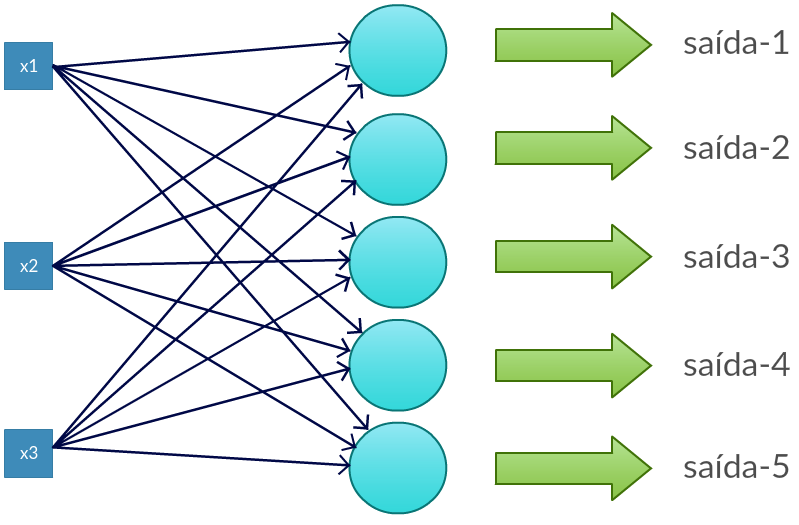
\includegraphics[width=0.6\textwidth]{camadaunica}}
	\caption{Representação de uma Rede Neural Artificial com camada única}
	\fonte{Elaborado pelo autor}
	\label{exec-rna-camada-unica}
\end{figure}

Para exemplificar este modelo de camada única, pode-se citar a RNA \textit{Perceptron} simples, criada por Frank Rosenblatt em 1957 nos laboratórios das forças militares. A classificação dos resultados de uma RNA desta categoria é ilustrada na Figura 5, onde seus resultados são linearmente separáveis, ou seja, este modelo de RNA é capaz de classificar de forma satisfatória, resultados que podem ser separados por uma reta ou hiperplano como fronteira de decisão \cite{haykin2009}.

\begin{figure}[h]
	\centering
	\fbox{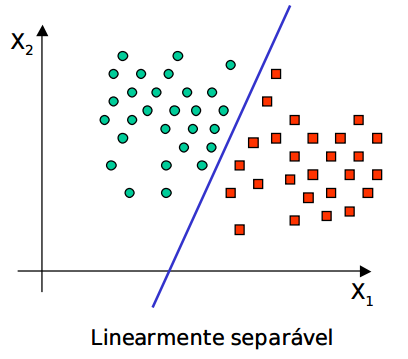
\includegraphics[width=0.5\textwidth]{separavel}}
	\caption{Representação de resultados linearmente separáveis}
	\fonte{\citeonline{oliveira2002} }
	\label{exec-linearmente-separavel}
\end{figure}

\subsection{Redes Alimentadas Adiante com Múltiplas Camadas}
A estrutura de múltiplas camadas, difere-se da primeira classe alimentada adiante em relação a composição de suas camadas. Esta classe de redes surgiu da necessidade em aperfeiçoar a capacidade de mapeamento que um modelo de camada única não proporciona. Um exemplo clássico é a função ou-exclusivo (XOR) \cite{haykin2009}.

Tipicamente, a rede consiste em uma camada de entrada, uma ou mais camadas ocultas e uma camada de saída. O sinal de entrada se propaga para frente através da rede, camada por camada. Este tipo de rede é bastante popular devido aos métodos de aprendizado bem distribuídos e de fácil uso \cite{haykin2000}.

Sua representação pode ser vista na Figura 6, onde pode-se observar a presença de duas camadas intermediárias até a apresentação de seu resultado.

De acordo com \citeonline{haykin2000}, qualquer rede semelhante à representada na Figura 6, é dita totalmente conectada, visto que todas as entradas $x_i$ se conectam a todos os nós da camada oculta $a_i$. Caso a premissa não fosse estabelecida a rede seria dita parcialmente conectada.

Outro ponto que a difere da classe com camada única, é a possibilidade de trabalhar com problemas não-lineares, ou seja, os resultados não necessariamente são classificados de forma satisfatória através apenas de uma reta ou hiperplano, o que aumenta a capacidade de RNAs com esta característica em resolver problemas mais complexos.

\begin{figure}[h]
	\centering
	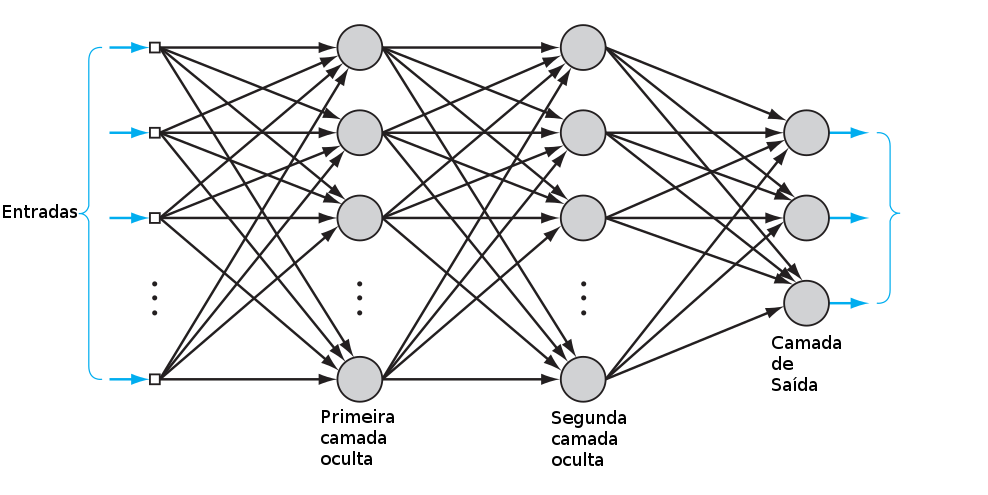
\includegraphics[width=0.9\textwidth]{multicamada}
	\caption{Rede Neural Artificial com múltiplas camadas}
	\fonte{Adaptado de \citeonline{haykin2009}}
	\label{fig-multiplas-camadas}
\end{figure}

A Figura 7 exemplifica a representação de um resultado não-linear proporcionado por uma rede de múltiplas camadas.

\begin{figure}[h]
	\centering
	\fbox{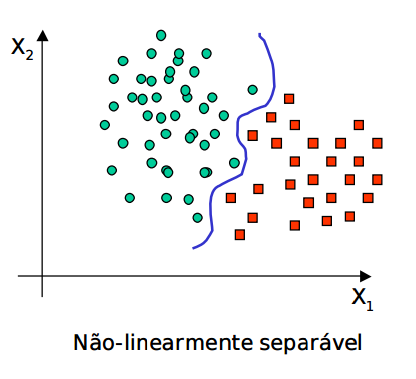
\includegraphics[width=0.5\textwidth]{naolinear}}
	\caption{Classificação de resultados não-lineares}
	\fonte{\citeonline{oliveira2002}}
	\label{exec-nao-linear-imagem}
\end{figure}

\subsection{Redes de Camadas Recorrentes}
Diferentemente da arquitetura de camadas simples adiante, a arquitetura de camadas recorrentes apresenta ao menos um laço de realimentação. A presença de realimentação de informação permite a criação de representações internas e dispositivos de memória capazes de processar e armazenar informações temporais e sinais seqüenciais. Em seu trabalho, \citeonline{haykin2000} cita um exemplo clássico de uma rede de camadas recorrentes, onde os neurônios em camada única alimentam seus sinais de saída novamente para as entradas de todos os neurônios.

A arquitetura de uma RNA recorrente pode ser observada na Figura 8, onde as entradas são realimentadas através da saída. Após realizado esse processamento, a rede apresenta o resultado calculado.

\begin{figure}[h]
	\centering
	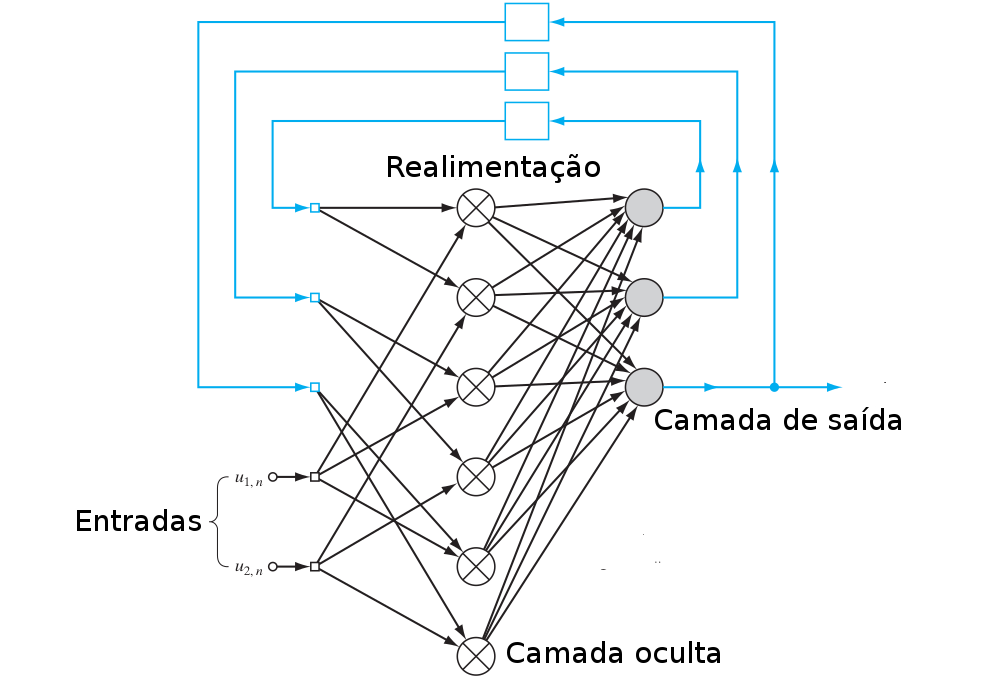
\includegraphics[width=.9\textwidth]{recorrente}
	\caption{Rede Neural Artificial recorrente}
	\fonte{Adaptado de \citeonline{haykin2009} }
	\label{fig-recorrente}
\end{figure}

\subsection{Redes de Hopfield}
Dentre outros modelos e arquiteturas de redes que existem, pode-se citar Hopfield, desenvolvida pelo físico John Hopfield. Este modelo se caracteriza por ser do tipo \textit{feedback}, por este motivo, estas redes dificilmente chegam a um estado instável, pois chegará um momento, após seu treinamento, em que o valor de saída para determinadas entradas se padronizam, alcançando sua estabilidade. O modelo utilizou uma função de energia como ferramenta para desenhar redes recorrentes e entender como funciona seu comportamento dinâmico. Desta forma, popularizou o uso desta arquitetura como uma memória associativa e para resolver problemas de otimização \cite{cardon}.

O modelo aplica um princípio chamado de armazenamento de informação como atratores dinamicamente estáveis. Para recuperar informações, utilizou um processo dinâmico de atualização dos estados dos neurônios, sendo que, o neurônio a ser atualizado, é escolhido aleatoriamente. Dois modelos de redes foram apresentados por Hopfield: o analógico e o binário \cite{silva}.

\subsection{Redes Auto-Organizáveis}
Segundo \citeonline{haykin2009}, Redes Auto-Organizáveis são modelos de 2 camadas que aceitam padrões de N-dimensões como entrada e os mapeia para um conjunto de neurônios de saída, o qual representa o espaço dos dados a serem agrupados. O mapa (camada) de saída, que é tipicamente bi-dimensional, representa as posições dos neurônios em relação aos seus vizinhos. A ideia é que neurônios topologicamente próximos respondam de maneira semelhante a entradas semelhantes. Para isso todos neurônios da camada de entrada são todos conectados aos neurônios de saída.

\section{FUNÇÃO DE ATIVAÇÃO}\label{sec:funcao-ativacao}
O processamento em cada neurônio se dá através da função de ativação. A escolha da função de ativação de uma RNA é um processo de grande relevância, uma vez que esta função define como devem ser tratados seus dados de entrada. As funções de ativação podem ser classificadas como lineares ou não lineares \cite{haykin2000}.

Segundo \citeonline{haykin2000}, caracterizando-se pela limitação de valores de saída a um intervalo finito, destacam-se os modelos de funções: limiar, sigmóide e tangente hiperbólica.

\subsection{Função Limiar}
Para este exemplo de função, o seguinte cálculo deve ser utilizado:
\begin{equation}\label{eq:limiar}
y=\sum_{j=1}^{w} w_{kj}\ x_j + b_{k'},
\end{equation}
onde $x$ é a entrada induzida no neurônio, gerando um resultado $y_k$ dado por:
\begin{equation}\label{eq:limiar-result} 
y_k = {1\ se\ x_j  > 0}
\end{equation}
ou
\begin{equation}\label{eq:limiar-result} 
y_k = {0\ se\ x_j < 0}  
\end{equation}

Neste modelo a saída do neurônio assume o valor 1 se o campo local induzido daquele neurônio for positivo, e 0 se for negativo. Utilizam-se dos mesmos preceitos de regressão linear e de outras técnicas, para estimar resultados a partir de valores conhecidos.

\subsection{Função Sigmóide}
A função sigmóide, representada na equação (3.4), é a forma mais comum de função de ativação utilizada na construção de RNAs.
\begin{equation}\label{eq:limiar-result} 
f(x)=\frac{1}{1+e^{- \lambda x}} ,
\end{equation}
onde $- \lambda x$ é a entrada a ser processada.

\citeonline{haykin2009} define a função sigmóide como uma função crescente, com o objetivo de realizar um balanceamento adequado entre comportamentos lineares e não-lineares em um intervalo entre [0,1], justificando sua grande usabilidade. No Código 1 é apresentada a implementação da função na linguagem de programação Python.

\citeonline{haykin2009} também evidência a utilização da tangente hiperbólica com o mesmo intuito da sigmóide, porém com um intervalo variando em um intervalo de [-1,1].
\codigoPython\
\lstinputlisting[label=cod:exempla-sigmoide, caption=Função sigmóide em Python]{src/Sigmoide.py}

Resultados com esta característica são reconhecidos por formar um "S", exemplificado no Gráfico 1.

\begin{grafico}[h]
	\centering
	\fbox{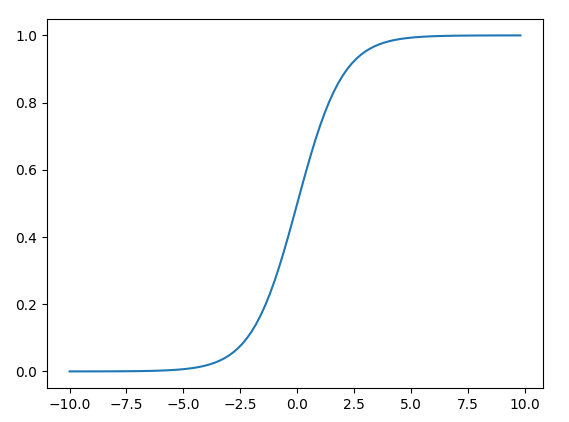
\includegraphics[width=0.8\textwidth, height=0.33\textheight]{sigmoide}}
	\caption{Comportamento de uma função sigmóide}
	\fonte{Elaborado pelo autor}
	\label{sigmoide-graph}
\end{grafico}


\section{TREINAMENTO DE UMA REDE NEURAL ARTIFICIAL}\label{sec:rna-treinamento}
Após determinar a arquitetura a ser utilizada pela RNA, a quantia de camadas, a função de ativação adequada ao trabalho a ser realizado, a rede neural deve adquirir conhecimento em relação aos dados aplicados sobre a mesma.

O treinamento de uma RNA consiste em minimizar uma função de custo, através de um algoritmo, cujos valores iniciais são escolhidos aleatoriamente com o objetivo de facilitar a busca  pelo valor mínimo da função da amostra de treinamento, através de iterações. O treinamento pode ser interrompido de duas formas: Um limite de épocas estipulado para o treinamento ou um ponto de parada a partir de um critério de desempenho.

Os critérios de desempenho típicos em um processo de treinamento, de uma determinada amostra de dados, são o Erro quadrático médio (EQM), Raiz do Erro Quadrático Médio (REQM) e o Erro Absoluto Médio (EAM) \cite{gambogi}. 

\subsection{Processo de Aprendizagem}
O processo de aprendizagem é considerado uma etapa de grande dificuldade em termos de análise de dados, porque a procura da solução adequada ocorre em um universo de soluções válidas de grande dimensão, onde a base de tomada de decisão serão os próprios dados treinados \cite{medeiros}.
 
Para adquirir conhecimento, uma RNA requer um processo de inúmeras iterações e aprendizagem, absorvendo os conhecimentos sobre o comportamento e relacionamento dos dados a cada iteração e armazenando os ajustes realizados nos pesos sinápticos de cada neurônio \cite{neto}.

Segundo \citeonline{haykin2000}, o processo de aprendizagem de uma rede neural pode ser resumido a uma sequência de três passos a cada estímulo enviado a rede, são eles:

\begin{enumerate}
	\item \textit O ambiente estimula a RNA com informações oriundas do mundo exterior;
	\item \textit A RNA experimenta alterações em seus pesos na tentativa de melhor responder ao estímulo recebido;
	\item \textit A RNA responde ao estímulo recebido após empreender as alterações realizadas no evento anterior.
\end{enumerate}

A cada estímulo enviado a RNA em sua aprendizagem, a sequência acima é realizada, os pesos sinápticos são ajustados até que atinjam seus valores ideais, visando aumentar a acuracidade dos resultados do processo, este processo, segundo \citeonline{haykin2000}, é conhecido como algoritmo de aprendizagem.

\subsubsection{Aprendizagem Supervisionada}
Nesse modelo de aprendizagem, o acompanhamento dos resultados é supervisionado constantemente durante o processo de treinamento e aprendizagem da rede. Nele, é disponibilizado o resultado esperado em relação aos dados aplicados na RNA, logo, estima-se a qualidade dos resultados obtidos de acordo com alguma métrica estabelecida, como, por exemplo, o desvio do padrão de resultados obtidos em relação aos aguardados \cite{haykin2009}.

Então, um algoritmo de aprendizagem supervisionada busca usar explicitamente a informação atual para, no futuro,  ser possível classificá-la como relevante ou não. O exemplo mais simples de um método baseado nesse tipo de aprendizagem é o modelo de regressão linear, quando estimado usando por exemplo a minimização dos erros quadráticos, isto é, a minimação do erro quadrático entre o valor da variável predita pelo modelo e o valor da variável real \cite{elpink}.

\subsubsection{Aprendizagem não Supervisionada}
No modelo de aprendizagem não supervisionada, não há supervisão dos dados processados, tal como não é disponibilizado um modelo de resultados esperados na aplicação em questão.

Segundo \citeonline{haykin2009}, dentre as existentes destacam-se duas formas de aprendizagem não supervisionadas, são elas: aprendizagem por reforço e aprendizagem auto-organizada. A primeira delas está diretamente relacionada à métodos de programação dinâmica. Já a segunda, está relacionada a aprendizagem competitiva, método onde os neurônios são postos de forma que compitam entre si, sendo somente um deles ativado no ciclo de aprendizagem.

Portanto, esses métodos de aprendizagem não supervisionada podem ser utilizados em grandes quantidades de dados não estruturados para encontrar padrões existentes, e, a partir disso, realizar as devidas análises. Esta abordagem é bastante utilizada em aplicações de mineração de dados (\textit{datamining}), onde o conteúdo de grandes bases de dados não é conhecido antecipadamente \cite{elpink}.

\section{ALGORITMOS DE APRENDIZAGEM PARA TREINAMENTO DAS REDES}\label{algoritmos-aprendizagem}
Muitos algoritmos são aplicados para a minimização e melhoria da aprendizagem da RNA. Esses algoritmos podem ser classificados como de minimização local e minimização global. Algoritmos de minimização local, tal qual o método gradiente descendente, são rápidos, porém convergem para mínimos locais. Por outro lado, os algoritmos de minimização global utilizam métodos de busca para achar soluções aproximadas, como estratégias heurísticas e algoritmos genéticos, buscando não convergir para mínimos locais \cite{haykin2000}.

\subsection{\textit{Backpropagation}}
O algoritmo de retropropagação (\textit{backpropagation}) é um método baseado no gradiente descendente, de aprendizado supervisionado e com alimentação à frente, que utiliza a função de ativação do tipo sigmóide e um coeficiente de aprendizado, denominado \textit{learning rate}, responsável por especificar uma taxa de convergência da RNA, este coeficiente de aprendizado normalmente está em um intervalo entre [0,1]    \cite{haykin2000}.
Neste modelo, reconhecido por ser a técnica mais utilizada dentre os métodos de treinamento aplicados, o erro de saída obtido se propaga para as camadas intermediárias da RNA, isso se dá pela necessidade de ajuste dos neurônios que não tem contato com a saída, possibilitando assim, a atualização dos pesos desses neurônios, aumentando o poder de classificação e de correção de erros \cite{medeiros}.

O algoritmo usa a equação abaixo para atualizar os pesos de um determinado neurônio.
\begin{equation}\label{eq:backpropagation-ajuste-pesos}
W_{ij,(t+1)} = W_{ij, t} + (\lambda)(\varepsilon W_{ij})(N_i)
\end{equation}

A equação (3.5) realiza a atualização do peso $W_{ij}$ de um determinado neurônio $N_i$ referente ao neurônio atual $N_j$ , onde o sub-índice $t$ refere-se ao número de vezes em que a rede foi atualizada e $\lambda$ refere-se à taxa de aprendizagem (\textit{learning rate}). Esta taxa de aprendizagem é responsável por controlar o peso e suas alterações.

Como dito anteriormente, o algoritmo trabalha com a função de ativação sigmóide para tratar suas saídas, a equação (3.4) representa o cálculo realizado pela função.

Após organizar os dados da saída da rede, é necessário ajustar os pesos caso haja um erro na resposta esperada, este cálculo de erro é detalhado na equação (3.6)
\begin{equation}\label{eq:backpropagation-calculo-erro}
E_j = \frac{1}{2} \sum_{saidas} (N_j - D_j)^2,
\end{equation}
onde $D_j$ é a saída desejada e $N_j$ é o resultado atual do neurônio. 	

Encontrando o valor do erro, é necessário calcular a variação do mesmo em relação às mudanças dos valores de entrada, isso é feito determinando quanto a equação (3.6) se altera em relação à equação (3.5). O cálculo é dado pela equação abaixo.
\begin{equation}\label{eq:backpropagation-calculo-erro-diferença}
\varepsilon S_{j} = E_j N_j (1 - N_j)
\end{equation}

O próximo passo é calcular os pesos ajustados para $W_{ij}$ da camada atual $N_i$ para o neurônio atual $N_j$. Abaixo é possível observar o cálculo deste procedimento.
\begin{equation}\label{eq:backpropagation-ajustes-erro}
\varepsilon W_{ij} = \varepsilon S_j N_i
\end{equation}

Por fim, a equação (3.9) é usada para calcular as atualizações dos pesos de cada neurônio $N_j$ ajustado, dada por:
\begin{equation}\label{eq:backpropagation-ajustes-erro-propagacao}
\varepsilon Hi = \sum_{j} \varepsilon S_{j}W_{ij},
\end{equation}
onde $j$ representa os neurônios da camada escondida.

De forma geral, as operações de cada neurônio seguem os cálculos especificados acima. A ideia é que os valores dos neurônios sejam atualizados de acordo com cada entrada da rede. 

\subsection{Algoritmo de Aprendizado Hebbiano}
O Aprendizado Hebbiano é uma classe de aprendizado não-supervisionado ou auto-organizado, onde uma RNA treinada sob este algoritmo possui capacidade de descobrir padrões significativos ou características em dados sem o auxílio de um padrão pré-definido, deixando a cargo da própria RNA aprender por sí só os padrões, características, correlações ou categorias nos dados de entrada \cite{castro}.

Segundo \citeonline{haykin2000}, o primeiro princípio do Aprendizado Hebbiano afirma que as modificações nos pesos sinápticos, baseadas em sinais pré-sinápticos e pós-sinápticos, tendem a se auto-amplificar. Uma sinapse forte leva à coincidência entre os sinais pré-sinápticos e pós-sinápticos e isto leva ao acréscimo da força da sinapse.

os sinais pré-sinápticos e pós-sinápticos, respectivamente x e y, podem ser equacionados por:
\begin{equation}\label{eq:hebbiano}
w_{0} (n + 1) = w_{0}(n)+ \eta y_0(n)x(n),
\end{equation}
onde $w_{0}(n)$ é o peso atual do neurônio, $\eta$ é a taxa de aprendizagem, $x(n)$ é a entrada da rede e $y_0(n)$ é a saída da rede.

\citeonline{castro} diz que o segundo princípio do Aprendizado Hebbiano trabalha através de competição entre os pesos sinápticos, ou seja, um aumento na força de algumas sinapses na rede deve ser compensado por um decréscimo em outras. Assim, só as sinapses de sucesso podem crescer, enquanto as de menos sucesso tendem a enfraquecer podendo, inclusive, desaparecer.

\section{PROCESSO DE GENERALIZAÇÃO}\label{rna-generalização}
O processo de generalização de uma RNA, ocorre a partir da sua capacidade em responder adequadamente não somente aos padrões de treinamento mas também aos demais padrões \cite{medeiros}. Vale ressaltar que o processo de treinamento é uma das eta	pas mais delicadas, em termos de análise e execução, ao se utilizar um modelo de RNA.

Tendo este conceito como ponto de partida, a capacidade de alta generalização desses modelos são fatores fundamentais para alcançar um nível de excelência. Desde os primórdios dessas técnicas, são utilizados métodos que possam abstrair a complexidade e suprir a necessidade de controlar o processo de generalização.

\subsection{Problemas de Generalização}
 Diferentes realizações para um conjunto de treinamento podem fazer com que diferentes soluções sejam tomadas, dada uma topologia de rede. Essa variabilidade de soluções, dados os conjuntos de treinamentos distintos para uma mesma tarefa, é chamada de variância \cite{haykin2000}.
 
Para garantir uma boa capacidade de generalização, a ideia é minimizar ao máximo essa variância que ocorre no processo de treinamento \cite{medeiros}. As inconsistências que influenciam  na capacidade de generalização de um algoritmo podem ser atribuídas aos seguintes fatores: sobre-ajuste (\textit{overfitting}), sub-ajuste (\textit{underfitting}) e sobretreinamento (\textit{overtraining}). A seguir encontram-se alguns detalhes a respeito desses fatores.

\subsubsection{\textit{Overfitting} e \textit{Underfitting}}
As soluções que apresentam inconsistências devido à alta taxa de variância geralmente apresentam sobre-ajuste em relação aos dados de treinamento, efeito conhecido como overfitting \cite{medeiros}. Na Figura 9 pode-se observar o comportamento de uma função com \textit{overfitting}.

Uma forma de evitar a alta taxa de variância, e assim, a ocorrência de \textit{overfitting}, se dá pela simplificação dos parâmetros de ativação da RNA. Porém, a redução desses parâmetros podem ocasionar outro problema muito comum dentre os protótipos desenvolvidos, denominado \textit{underfitting}. \textit{Underfitting} refere-se a um modelo que não pode nem modelar os dados de treinamento nem generalizar a novos dados, tornando-se um modelo estático, limitando assim, sua característica de aprender novos padrões \cite{geman}. Na Figura 9 pode-se observar o comportamento de uma função com \textit{underfitting}.

Com isso nota-se que deve existir um ponto de equilíbrio entre ambos efeitos, várias são as abordagens que tentam minimizar esses problemas, como os métodos construtivos e os algoritmos de \textit{pruning}.

Os algoritmos construtivos buscam a construção gradual da RNA por meio da adição, até que um critério de parada envolvendo o erro de treinamento seja atingido. A resposta da rede se inicia em uma situação de \textit{underfitting} e com a adição de novos neurônios aproxima-se de \textit{overfitting}, a ideia desses algoritmos consiste em encontrar uma melhor generalização na transição entre esses dois extremos \cite{medeiros}.

Os algoritmos de pruning, por sua vez, visam à minimização da estrutura pela eliminação gradativa dos pesos e dos neurônios, buscando diminuir os pesos excessivos, e assim, diminuindo o \textit{overfitting}.

\begin{figure}[h]
	\centering
	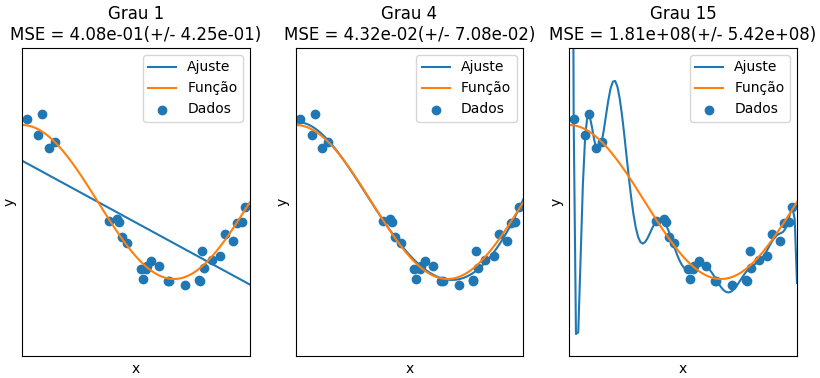
\includegraphics[width=0.9\textwidth]{overfitting}
	\caption{Comportamento de funções com \textit{overfitting} e \textit{underfitting}}
	\fonte{Elaborado pelo autor}
	\label{overfittin-fig}
\end{figure}

\subsubsection{\textit{Overtraining}}
As arquiteturas convencionais de treinamento estão sujeitas a sofrerem um sobretreinamento (\textit{overtraining}). Quando a rede parece estar respondendo o conjunto de dados cada vez melhor, ou seja, o erro de treinamento do conjunto de dados continua diminuindo, em algum ponto desse processo, a capacidade em resolver novos padrões torna-se falha. Isto ocorre por utilizar dados muito parecidos, assim como a quantidade de épocas em que esse conjunto de dados é treinado, viciando o conhecimento da RNA \cite{haykin2000}.

\section{TEORIA DA REGULARIZAÇÃO}\label{regularizacao}
A regularização é um método que busca melhorar a capacidade de generalização dos algoritmos de aprendizado por meio de alguma regra durante o processo de treinamento. A ideia básica da regularização é estabilizar a solução por meio de uma suavização entre o mapeamento da entrada até a saída, no sentido de que entradas similares correspondam a saídas similares. A suavização pode transformar um problema mal posto em um problema bem posto \cite{medeiros}. Um dos problemas a ser resolvido com métodos de regularização, seria encontrar um ponto de equilíbrio entre \textit{overfitting} e \textit{underfitting} no processo de treinamento de uma RNA, implicando na suavização do conjunto de dados.

\section{SÉRIES TEMPORAIS}\label{series-temporais}
Séries temporais são definidas como sequências de dados indexados ao longo de um período. Diferentemente de dados em seção transversal (\textit{cross-section}), em que os dados são coletados somente em um determinado instante de tempo, representando uma instância dos dados naquele momento, a ordem temporal dos dados tem relevância na obtenção de resultados e conclusões. Se a ordem dos dados for modificada, haverá perda de informação relevante sobre os dados, podendo obter conclusões equivocadas em relação à série em estudo \cite{neto}.

As séries temporais podem ser classificadas de diversas formas. Elas podem ser contínuas, quando a sequência de dados é descrita continuamente no tempo, e discretas, quando a sequência de dados é descrita em instantes de tempo discretos, havendo um espaçamento entre os instantes. A classificação em discreta e contínua é em relação ao tempo e não ao valor de cada observação. Pode-se ter uma série temporal discreta, mas o conteúdo das suas variáveis ser contínuo. Na prática, a utilização de séries temporais econômicas e financeiras é dada na forma discreta, pois, a coleta de dados é viabilizada em instantes de tempo discretos \cite{oliveira2012}.

\section{MERCADO DE CAPITAIS}\label{capitais}
O mercado de capitais é um sistema de distribuição de valores mobiliários que visa proporcionar liquidez aos títulos de emissão de empresas e viabilizar seu processo de capitalização. É constituído pelas bolsas, corretoras e outras instituições financeiras autorizadas \cite{tororadar}.

Os mercados de grandes ações são considerados os pilares centrais do crescimento e desenvolvimento econômico. Prever como irá se comportar futuramente o movimento de ações, tornou-se interesse comum entre investidores deste mercado \cite{pereira}.

Partindo deste pretexto, estudos ligados a predição de valores do mercado acionário, dividem-se basicamente em três vertentes. Há os que não crêem que investidores podem conseguir consideráveis vantagens em transações, que se fundamentam em teorias aleatórias de mercado. Há também os que crêem no hábito de seguir aspectos relacionados a análise fundamentalista de empresas e indicadores macro-econômicos. Por fim, há os que crêem que com base em séries recentes de dados e históricos é possível conseguir generalizar e classificar padrões de dados. A partir da última citação, surgem os interesses em trabalhos que relacionam o tema à técnicas de inteligência computacional, especificamente o uso de redes neurais artificiais \cite{pereira}.

\subsection{Análise Fundamentalista de Acões}
Antes da realização de qualquer investimento no mercado acionário é fundamental que sejam analisados itens de considerável importância no ramo financeiro, como indicadores de balanço e de mercado. O objetivo da análise é de reconhecer previamente as altas e baixas de determinadas ações em um período de tempo.

A análise fundamentalista busca, basicamente, avaliar a saúde financeira das empresas, projetar seus resultados futuros e determinar o preço justo para as suas ações. Para isso, os analistas levam em consideração os chamados fundamentos da empresa, isto é, todos os fatores macro e microeconômicos que influenciam no seu desempenho. A partir de uma minuciosa análise de todos eles, é possível projetar os resultados da companhia a longo prazo, em geral num período de cinco a dez anos \cite{exame}.

\subsection{Análise Técnica de Ações}\label{ch:analise-tecnica}
Análise Técnica de ações é a prática de medir as flutuações futuras do preço de uma ação analisando suas atividades passadas. Este método envolve a procura de padrões gráficos e o exame de outros dados históricos relacionados a preço e volume de ações negociadas \cite{tororadar}.
 
Relaciona as oscilações de preços do mercado em relação à ação, e não à empresa. Este modelo de análise acredita na repetitividade do comportamento humano e no poder da ciência estatística como forma de determinar, com base no comportamento passado, as perspectivas para o mercado no futuro \cite{pereira}.

A análise técnica também é conhecida como escola grafista, e auxilia o investidor na escolha do melhor momento para compra e venda de ações. Esta escola baseia-se na análise gráfica, tendo como base os volumes e os preços pelos quais foram comercializadas as ações nos pregões anteriores \cite{fortuna}.

Pensando dento deste contexto, não seria extremamente lucrativo saber qual lado está mais forte? O da demanda (compradores) ou da oferta (vendedores)? Esse é o trabalho da Análise Técnica de Ações.

Uma boa métrica para análise técnica se dá pela utilização de seus gráficos de preço das ações para encontrar padrões que indiquem quem está mais forte no mercado. Se existem sinais de que a demanda está forte e a oferta fraca pode ser uma bela oportunidade de comprar e ganhar com a alta, enquanto no cenário contrário pode ser que seja a hora ideal de se vender aquela ação \cite{tororadar}.

\subsection{Bolsa de Valores NASDAQ}
A bolsa de valores que será utilizada como referência para a execução do trabalho, será a  \textit{National Association of Securities Dealers Automated Quotations} (NASDAQ). Fundada em 1971, é atualmente a segunda maior bolsa de valores de mercado do mundo. Grande parte das empresas listadas no mercado de ações da NASDAQ, fazem parte do ramo de produção de alta tecnologia, como o Facebook, Apple, Amazon, Adobe, Cisco, dentre outras, incluindo a própria NASDAQ, listada em seu mercado desde 2002. 
A NASDAQ é muito conhecida pela realização de negócios de mercado inteiramente de forma eletrônica. O mercado financeiro considera o conjunto de negócios realizados através da NASDAQ como Nova Economia, o que a difere da Bolsa de Valores de Nova York, por exemplo, considerada como Velha Economia \cite{christie}.

% !TeX encoding = UTF-8

\chapter{MATERIAIS E MÉTODOS}\label{ch:materiais-metodos}
Conforme mencionado anteriormente, o objetivo principal dessa dissertação é especificar e aplicar um modelo de RNA para análise e predição de valores acionários. Neste capítulo será realizada a pergunta de pesquisa e dos objetivos do trabalho na escolha da metodologia. Em seguida, esta metodologia será descrita e classificada quanto ao seu conteúdo e quanto aos métodos empregados na coleta e análise de dados.

\section{IDENTIFICAÇÃO DA PESQUISA}

Para se escolher a metodologia de pesquisa, alguns aspectos importantes precisaram ser analisados. Uma pesquisa pode ser realizada com dados criados ou com dados existentes. No primeiro caso, os dados são coletados após uma intervenção destinada a provocar uma mudança. No segundo, os dados estão presentes na situação em estudo e o pesquisador, por meio das técnicas de pesquisa, faz tais dados aparecerem, sem a intenção de modificá-los, através de uma intervenção. Na pesquisa experimental, delimita-se o fenômeno, formulam-se hipóteses, determinam-se os métodos e submete-se o fenômeno à experimentação em condições de controle \cite{laville}.

A escolha de uma estratégia de pesquisa tem que ser feita considerando-se, entre outros elementos, a natureza da questão da pesquisa, o contexto no qual a pesquisa se realizará, a formação e a experiência do pesquisador. De maneira geral, pode-se dividir as pesquisas em quantitativas ou experimentais e qualitativas \cite{laville}.

Portanto, de acordo com as afirmativas acima, a presente pesquisa é caracterizada por ser experimental e qualitativa. Segundo \citeonline{chizzotti}, na pesquisa experimental, o pesquisador parte de um estado delimitado a priori, sobre qual cria possíveis hipóteses que podem ser analisadas, determinando os métodos de verificação a serem utilizados, através dos quais procurará controlar as condições do experimento.

\section{SELEÇÃO DAS AÇÕES}
Para iniciar o processo de desenvolvimento deste trabalho, é necessário definir quais ações serão escolhidas para compor a implementação. Os critérios para definir quais serão selecionadas, são caracterizados pelo alto potencial de movimentação e lucratividade na NASDAQ, ou seja, são as empresas que mais influênciam na ecônomia, que, por coincidência, são do ramo da tecnologia \cite{christie}.

Tendo em vista os critérios especificados acima, as empresas selecionadas e o código de suas ações para a realização da coleta dos dados são:
\begin{itemize}
	\item Apple (AAPL);
	\item Amazon (AMZN);
	\item Cisco Systems (CSCO);
	\item Intel (INTC);
	\item Microsoft (MSFT);
\end{itemize}

\section{TÉCNICA PARA COLETA DE DADOS}
Com a definição da bolsa de valores em questão e das empresas que serão utilizadas para realizar a implementação deste trabalho, a próxima etapa se dá pela necessidade em coletar seus dados histórios.

Como os dados históricos das ações caracterizam-se por serem séries temporais, o tipo de técnica aplicada para conseguir indicadores de relevância para uma boa análise dos objetivos propostos, refere-se à análise técnica. 

Portanto, esta fase de coleta de dados é muito importante para o bom funcionamento da RNA que será criada, tornando-se essencial para o êxito final do trabalho.

\subsection{Definição das séries}
Selecionar os dados corretos para trabalhar com RNAs é uma fase de grande relevância, pois são esses dados que serão treinados e que irão garantir a estabilidade e a capacidade de generalização da rede em sí.

Sendo assim, a partir do conhecimento concebido pelo Capítulo 3, pode-se destacar dois aspectos importantes para a análise de quais dados coletar dentro de um problema em geral, sendo eles:

\begin{enumerate}
\item Dados que influeciam diretamente no resultado final e na coêrencia da análise proposta;
\item Uso de múltiplas séries de um mesmo dado para que a rede não se sujeite à \textit{overfitting} ou \textit{underfitting}.
\end{enumerate}

Segundo \citeonline{tororadar}, as variáveis que influenciam em um sistema de análise técnica das ações são:

\begin{enumerate}
\item Abertura: Valor da ação no ínicio do dia;
\item Máximo: Valor máximo negociado no dia;
\item Mínimo: Valor mínimo negociado no dia;
\item Volume: Número de negociações do papel no dia (valor bruto das negociações);
\item Valor de fechamento no dia;
\item Médias móveis simples: As médias móveis suavizam os dados de preços para formar um indicador de tendência sequencial. Elas não prevêem a direção dos preços, mas, antes, definem a sua direção atual com um atraso. Como o próprio nome indica, uma média móvel é uma média que se move. Os dados antigos são retirados, a medida que dados mais recentes se tornam disponíveis, isto faz com que a média se mova ao longo do tempo. A maioria das médias móveis são baseadas em preços de fechamento;
\item \textit{Moving Average Convergence Divergence} (MACD): indicador que controle a divergência e convergência das médias móveis. o MACD é formado pela diferença entre duas médias móveis, sendo uma de longo prazo e outra de curto prazo. Para o presente trabalho será calculado o MACD referente às médias de 10 e 26 dias.
\end{enumerate}

\section{FERRAMENTAS PARA COLETA DE DADOS}
Com a especificação das séries que serão coletadas, é necessário preparar um ambiente que dispõe o acesso à esses dados de forma simplificada. 

Pensando nesse contexto, é essencial utilizar uma linguagem de programação que tenha suporte à esse modelo de busca por dados. Tendo em vista essa premissa, a disponibilidade de uma API ou biblioteca é de extrema importância para a automatização deste processo.

\subsection{Linguagem de programação Python}
Segundo \citeonline{python-science}, apesar das diversas linguagens de programação disponíveis hoje para o desenvolvimento de aplicações e \textit{scripts}, a linguagem de programação Python vêm se destacando e crescendo constantemente na comunidade científica, seja por sua variedade de bibliotecas que auxiliam os desenvolvedores e pesquisadores à resolverem seus problemas de forma mais simplificada, até seu poder computacional e suas características de multiplataforma e multiparadigma.

Um fator que determina a utilização da linguagem de programação Python, como dito no paragrafo anterior, se dá pela sua variabilidade de bibliotecas voltadas, principalmente, para a análise de dados. Colocando isso no contexto deste trabalho, é essencial o uso de uma ferramenta que proporcione um alto nível de funcionalidades disponíveis para serem exploradas.

\subsection{Biblioteca pandas}\label{pandas-lib}
A biblioteca pandas é um pacote disponível na linguagem de programação Python que fornece fácil acesso à dados disponíveis na internet. O objetivo principal do pandas é justamente fornecer buscas flexíveis e intuítivas para a análise de dados estruturados e não estruturados. A biblioteca tem como objetivo específico se tornar a ferramenta de análise, busca e manipulação de dados aberta mais poderosa e flexível existente \cite{pandas}.

Segundo \citeonline{pandas}, o seu uso é adequado para diferentes tipos de dados, sendo eles:
\begin{enumerate}
\item Dados tabulares com colunas, como em uma tabela \textit{Structured Query Language} (SQL) de um banco de dados relacional ou uma planilha do Excel;
\item Dados de séries temporais não ordenados;
\item Qualquer outra forma de conjuntos de dados observacionais e estatísticos.
\end{enumerate}

Portanto, a principal justificativa para a utilização da biblioteca se dá pelo seu desenvolvimento, de código aberto, que impulsiona a comunidade a realizar diferentes aplicações, além da sua excelente documentação e suporte de acesso aos dados históricos da bolsa de valores NASDAQ, que são requisitos para a realização deste trabalho.

Para exemplificar como a biblioteca facilita o processo de coleta dos dados, o Código 2 ilustra uma pesquisa das ações da Microsoft, no período de 05/03/2001 a 11/04/2001.
\codigoPython\
\lstinputlisting[language=Python, label=script-coleta-dados, caption=\textit{Script} para coleta de dados]{src/microsoft.py}

As séries históricas são disponibilizadas em arquivos com valores separados por vírgulas (*.csv) contendo a data de negociação, valor de abertura, valores máximo e mínimo atingidos, valor de fechamento e o volume de negociações.

Na Figura 10 é possível observar o arquivo criado a partir do Código 2, demonstrando o formato especificado acima que a API retorna para a manipulação.

\begin{figure}[h]
	\centering
	\fbox{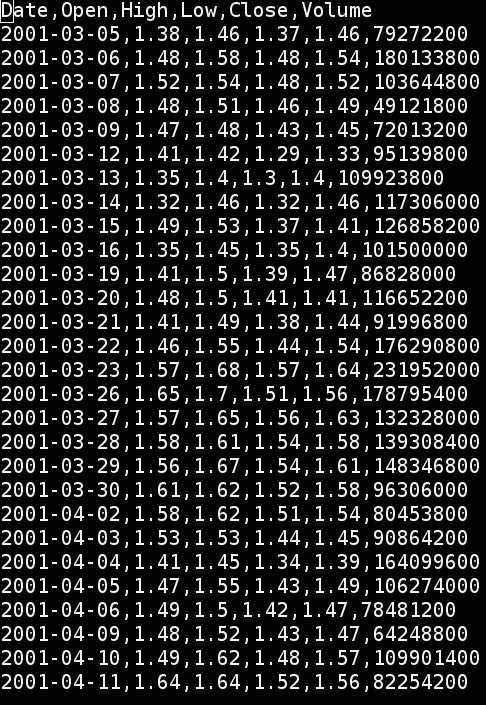
\includegraphics[width=0.5\textwidth, height=0.33\textheight]{dados-pandas}}
	\caption{Representação dos dados coletados pela biblioteca pandas}
	\fonte{Elaborado pelo autor}
	\label{exec-coleta-dados}
\end{figure}

\subsection{Google \textit{Finance} API}
É importante citar qual a fonte onde o pandas busca as séries históricas, por questões como confiabilidade dos dados. O acesso é realizado através da integração com o Google \textit{Finance} API, um banco de dados quase em tempo real mantido pelo Google, que trabalha com as principais bolsas de valores do mundo \cite{pandas}.

A API trabalha com um limite inicial para a coleta das ações, este limite se inicia em 03/05/2001 e vai se atualizando diariamente. Tendo em vista que para trabalhar com RNAs é importante buscar o máximo de informações possíveis e, também, considerando o limite disponível pela API, o período das ações das empresas selecionadas serão coletadas iniciando no ano de 2001 até o ano de 2017. 

Sendo assim, a ideia é preparar um ambiente que proporcione o uso dessa ferramenta, junto à biblioteca citada na \autoref{pandas-lib} para realizar a busca pelos dados necessários.

\subsection{PyCharm IDE}
É necessário utilizar uma \textit{Integrated Development Environment} (IDE) para auxiliar no \textit{script} de coleta de dados. PyCharm é uma IDE proprietária do grupo JetBrains que conta com uma versão livre para estudantes, que será realizada neste trabalho.
 
PyCharm suporta o desenvolvimento com a linguagem de programação Python desde a sua versão 2.4 até a versão 3.6. Vale citar que outras IDEs para o desenvolvimento poderiam ser utilizadas, porém a praticidade e a boa documentação das ferramentas JetBrains são fatores que justificam a sua utilização \cite{pycharm}.

\section{ESPECIFICAÇÃO DO MODELO DE REDES NEURAIS ARTIFICIAIS}\label{especifica-modelo}
Tendo como base o conhecimento adquirido no Capítulo 3, a definição de um modelo de RNA varia muito, sendo específico para cada problema do mundo real. Por isso, é importante frisar que não existe um modelo pré-definido e eficiente em RNAs, ficando a cargo da análise dos resultados, e, muitas vezes, por métodos de tentativa e erro para se chegar à um resultado eficiente \cite{haykin2000}.
 
Porém, com o estudo realizado no Capítulo 3, esse processo pode ser menos custoso do que parece. Avaliar o problema em que se está trabalhando junto com o conhecimento teórico é de grande auxílio para a especificação e construção de um modelo inicial que se aproxime do desejado.

Para especificar quais modelos não devem ser aplicados, ou seja, modelos que não tenham características referente a resolução do problema em questão, algumas perguntas-chave serão elaboradas, sendo elas:

\begin{enumerate}\label{enumerate-questions}
\item "Qual o modelo de dados se está trabalhando?";
\item "Estes dados serão treinados a partir de resultados esperados?";
\item "A RNA será exposta à uma quantidade significativa de dados desconhecidos aos treinados?".
\end{enumerate}

A primeira pergunta refere-se ao modelo de transmissão dos dados que a RNA deve implementar, ou seja, se ela será formada por camadas adiante ou recorrente. Como é necessário o ajuste dos pesos nas camadas intermediárias, após a saída, a RNA deverá trabalhar com um modelo de camadas recorrente.

A segunda pergunta refere-se ao processo de aprendizagem. Se os dados são treinados com resultados esperados, a RNA deverá possuir um método de aprendizado supervisionado, caso contrário, um modelo de RNA com treinamento não supervisionado deverá ser utilizado. A RNA será treinada a partir dos resultados esperados através das séries temporais, ou seja, o modelo trabalhará com aprendizagem supervisionada.

A terceira pergunta refere-se à capacidade de generalização. Sendo assim, um modelo de RNA que irá trabalhar com dados desconhecidos deve ter caracteristícas de boa generalização, caso contrário, um modelo simples já é o suficiente.

\subsection{Definição da Arquitetura}

Tendo em vista estes critérios estabelecidos na Seção anterior, chega-se a definição de que a RNA deverá possuir uma arquitetura de camadas recorrente, um método de aprendizado supervisionado e uma função de custo, para controlar o processo de generalização da mesma.

\citeonline{haykin2000} direciona este modelo de rede ao Perceptron de Múltiplas Camadas (MLP, \textit{Multilayer Perceptron}), são redes neurais compostas por um conjunto de unidades sensoriais que constituem a camada de entrada, uma ou mais camadas ocultas e uma camada de saída, onde o sinal de entrada se propaga para frente através da rede, camada por camada. Redes MLP trabalham normalmente junto ao algoritmo \textit{backpropagation} para realizar seu treinamento e aprendizado.

Tendo em vista a especificação do modelo da rede e dos dados que serão utilizados para realizar o treinamento e os testes, a próxima etapa será definir quais serão as entradas utilizadas. Como o objetivo do trabalho é realizar a predição do valor de fechamento das ações, todas as váriaveis coletadas, com a exceção do valor de fechamento, serão utilizadas como entrada da RNA. 

Portanto, as variáveis que irão compor a camada de entrada da RNA são:

\begin{enumerate}
\item Valor de abertura;
\item Valor máximo negociado no dia;
\item Valor mínimo negociado no dia;
\item Número de negociações do papel;
\item Média móvel simples de 10;
\item Média móvel simples de 26;
\item \textit{Moving Average Convergence Divergence} (MACD).
\end{enumerate}

Segundo \citeonline{haykin2000} e \citeonline{marangoni}, na camada intermediária da RNA existe um cuidado especial para especificar sua composição, pois o número de neurônios depende de várias condições, tais como:

\begin{itemize}
\item Quantidade de dados para treinamento em relação a quantidade de neurônios na camada oculta: Deve-se ter cuidado para não utilizar neurônios e camadas demais, o que pode levar a rede a memorizar os padrões de treinamento, quebrando seu processo de aprendizagem (\textit{overfitting}). O inverso também é válido, poucos neurônios para uma grande quantidade de dados, pode levar a rede a não encontrar uma solução desejável, pelo pouco poder de processamento (\textit{underfitting});
\item Definir o número de neurônios em função da dimensão das camadas de entrada e saída da rede: Pode-se definir o número de neurônios na camada escondida como sendo a média aritmética entre o tamanho da entrada e da saída da rede;
\item Utilizar um número de sinapses dez vezes menor que o número de exemplos disponíveis para treinamento.
\end{itemize}

Por isso, para a grande maioria dos problemas utiliza-se apenas uma camada escondida, onde sua quantidade de neurônios é definida buscando um meio termo entre a quantidade de entradas e a sua saída, tentando evitar as complicações evidenciadas nos tópicos anteriores.

Levando isso em consideração, a rede será desenvolvida com apenas uma camada intermediária composta por 11 neurônios, buscando otimizar a sua estrutura e obtendo um resultado eficiente para o problema.

Por fim, a saída da rede será composta por uma única camada que irá conter o valor do fechamento diário das ações. É importante deixar claro que este valor, durante o processo de treinamento, será preenchido com os valores reais das ações em relação ao período que será escolhido para o processo de treinamento. Na Figura abaixo é possível visualizar a composição gráfica da arquitetura proposta.

\begin{figure}[h]
	\centering
	\fbox{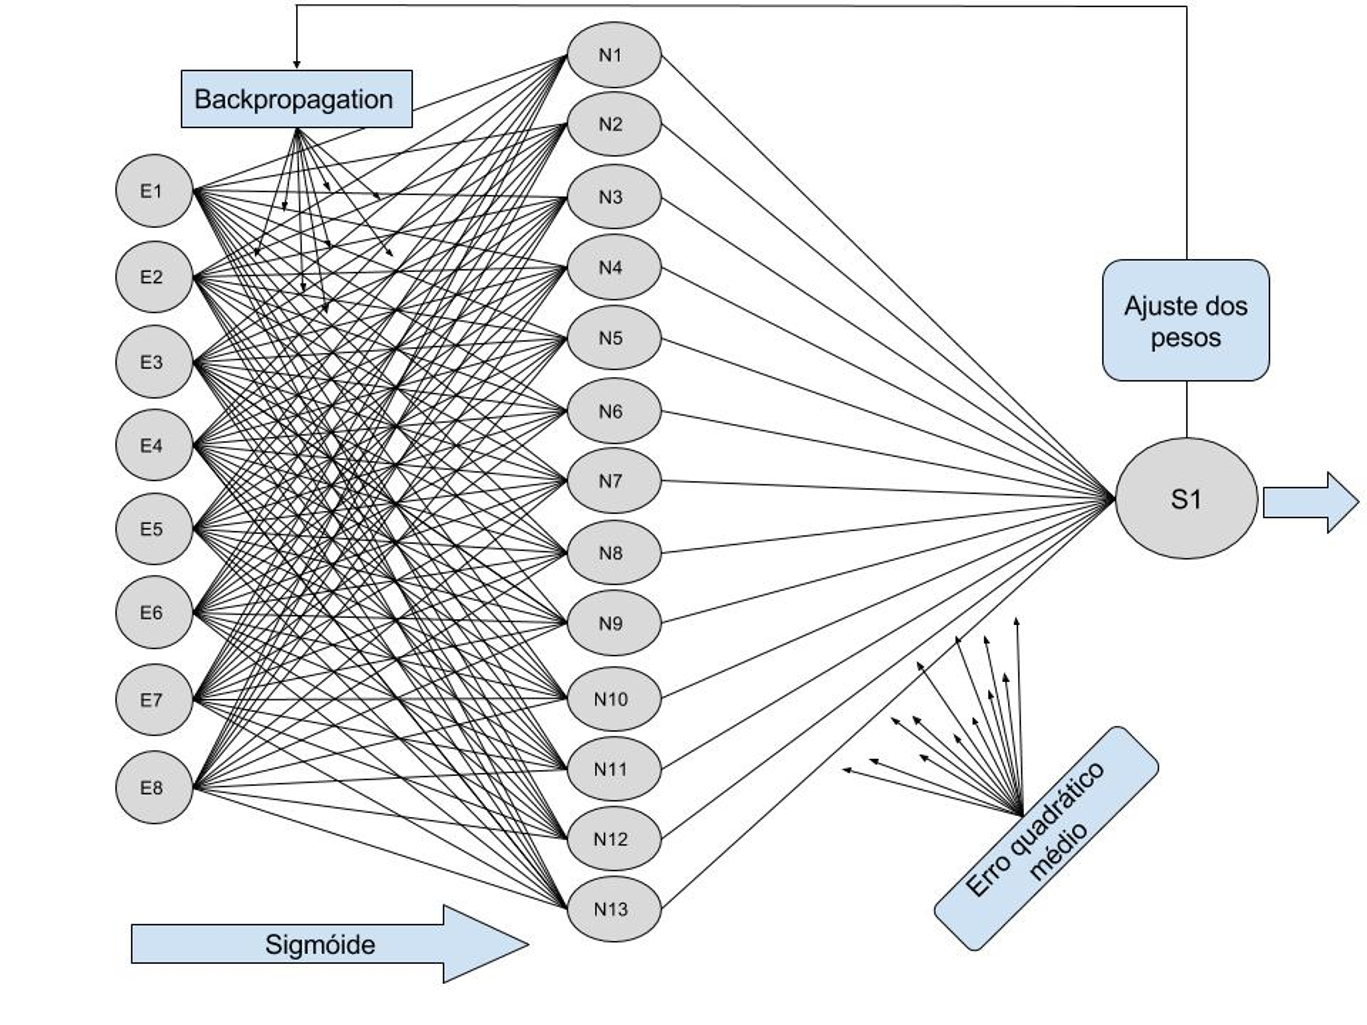
\includegraphics[width=0.8\textwidth, scale=0.5]{arquitetura-rna}}
	\caption{Modelo de arquitetura proposta utilizando o algoritmo \textit{backpropagation}}
	\fonte{Elaborado pelo autor}
	\label{exec-rna}
\end{figure}

\section{DEFINIÇÃO DA BASE DE TREINAMENTO}
A partir do modelo de rede definido, é necessário classificar os dados que serão utilizados na fase de treinamento e os que serão utilizados para a realização dos testes. Como no trabalho serão coletadas as ações de 5 empresas distintas, a ideia é que para cada empresa, individualmente, sejam realizados os processos de treinamento e testes, com objetivo de observar o comportamento da rede nas mais diversas situações e proporcionar uma análise mais detalhada do modelo.

Os dados utilizados para o treinamento da rede devem ser significativos e cobrir amplamente o domínio do problema, e não apenas envolver os casos de operações normais ou rotineiras, mas também incorporar casos de exceção e de situações limites. Seguindo o funcionamento do algoritmo \textit{backpropagation}, os dados treinados devem seguir os seguintes passos:

\begin{enumerate}
\item Aplicar o vetor de entrada da rede;
\item Calcular a saída da rede;
\item Ajustar os pesos da rede de maneira a minimizar o erro;
\item Repetir o passo (1) até o passo (3) para cada vetor do conjunto de treinamento, até que o erro (função de custo) seja satisfeito. 
\end{enumerate}

Segundo \citeonline{haykin2000}, ao determinar a classificação de um conjunto para treinamento, devem ser levados em consideração os seguintes fatores:

\begin{itemize}
\item Quando há uma grande quantidade de amostras disponíveis para o treinamento, a divisão deve se aproximar de 33\% para treino e 67\% para testes;
\item Quando o número de amostras é reduzido deve-se diminuir a proporção do conjunto de testes, com um valor próximo de 60\% para treinamento e 40\% para testes;
\item Em casos com um número muito pequeno de amostras, é recomandável utilizar 50\% para ambos.
\end{itemize}

\section{BIBLIOTECA PyBrain}
\textit{Python-Based Reinforcement Learning, Artificial Intelligence and Neural Network Library} (PyBrain) é uma biblioteca de aprendizagem de máquinas para Python. Seu objetivo é oferecer algoritmos flexíveis e fáceis de usar que proporcione uma forma mais intuitiva de desenvolver algoritmos complexos relacionados a Inteligência Artificial. Embora existam poucas bibliotecas de aprendizado de máquinas, PyBrain pretende ser uma biblioteca modular fácil de aprender, podendo ser utilizada por estudantes de nível básico até um nível mais avançado, oferecendo flexibilidade e algoritmos para pesquisa de ponta \cite{pybrain2010}.

Segundo \citeonline{pybrain2010}, como o próprio nome sugere, PyBrain contém algoritmos para redes neurais, aprendizagem supervisionada, aprendizagem não supervisionada e algoritmos evolutivos. A biblioteca é construída com seu núcleo baseado em redes neurais, onde todos os métodos de treinamento aceitam uma rede como instância pré-treinada. Isso faz de PyBrain uma ferramenta poderosa para a execução de tarefas complexas de serem resolvidas.

A Figura 12 demonstra de maneira mais clara como a biblioteca PyBrain irá auxiliar no projeto.

\begin{figure}[h]
	\centering
	\fbox{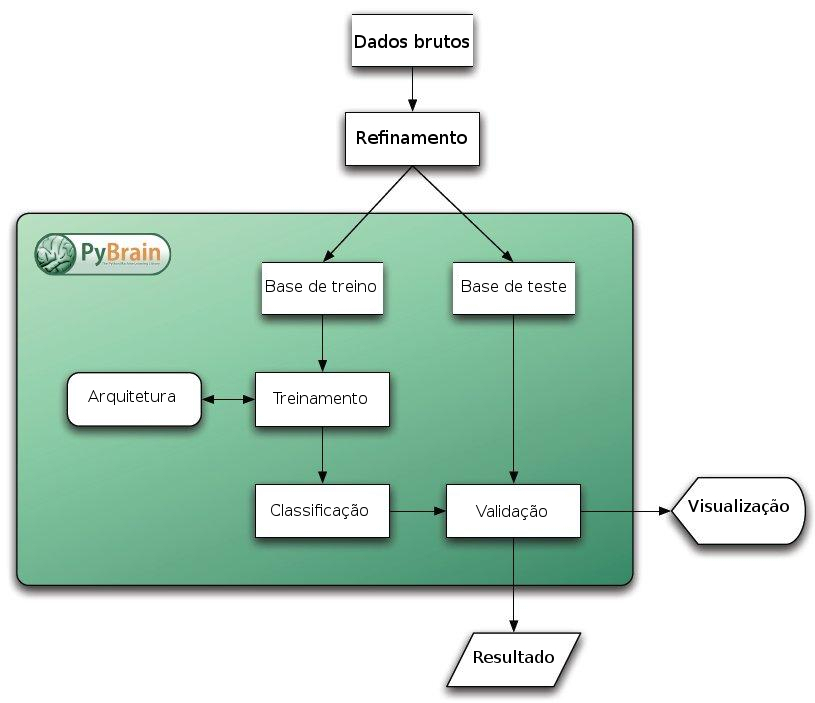
\includegraphics[width=0.8\textwidth, scale=0.5]{pybrain8}}
	\caption{Arquitetura da biblioteca PyBrain aplicada na estrutura do trabalho}
	\fonte{Adaptado de \citeonline{pybrain2010}}
	\label{exec-rna-pybrain}
\end{figure}

PyBrain tem ênfase nas arquiteturas de rede, que podem ser treinadas e manipuladas com quase todos os algoritmos oferecidos de aprendizado de máquina. As redes são compostas por módulos que estão ligados através de conexões, onde os nós são os módulos e as bordas são as conexões. Isso torna o PyBrain muito flexível, mas também necessário em todos os casos, seguir este padrão.

Alguns exemplos de arquiteturas disponibilizada pela biblioteca são:

\begin{itemize}
	\item Redes Neurais Alimentadas Adiante (\textit{Feedforward});
	\item Redes Neurais Recorrentes;
	\item Redes Neurais Recorrentes Multidimensionais;
	\item Redes de Kahonen (Mapas Auto-Organizáveis);
	\item Redes Bidirecionais;
	\item Topologias Personalizadas.
\end{itemize}

Dentre os algoritmos de aprendizagem supervisionada utilizado pelo PyBrain, destacam-se:

\begin{itemize}
	\item Algoritmo de retropropagação (\textit{backpropagation});
	\item Algoritmo de R-prop;
	\item Algoritmos de Máquinas de Vetores de Suporte (SVM).
\end{itemize}	

Também é importante evidenciar que a biblioteca PyBrain é de código aberto e gratuita para todos, licenciada sob a \textit{Berkeley Software Distribution} (BSD) Software.

Desta forma, todos os métodos necessários para realizar a implementação do trabalho foram levantados, o próximo capítulo será responsável por detalhar o processo de desenvolvimento das técnicas, e, consequentemente, da obtenção dos objetivos desejados, levando todos os aspectos estudados e definidos até o momento em consideração.
%% !TeX encoding = UTF-8

\chapter{IMPLEMENTAÇÃO DAS TÉCNICAS}\label{ch:implementacao}
Este capítulo tem como objetivo apresentar, de forma mais detalhada, todo o processo de implementação realizado no presente trabalho, com o intuito de alcançar os objetivos especificados no Capítulo 1.

\section{REALIZAÇÃO DA COLETA DE DADOS}
Tendo em vista as ferramentas necessárias para realizar à coleta das séries temporais que serão utilizadas para o treinamento e testes da RNA, foi desenvolvido um método de automatização de aquisição dos \textit{DataFrames} das ações que serão coletadas para a análise.

Inicialmente, foi criada uma interface em Python que contém a assinatura do método que as classes das empresas deverão implementar. Após isso, criou-se as classes para as respectivas empresas, definidas no Seção 4.2. Para exemplificar o que está sendo exposto, o Código 3 demonstra, de forma mais intuitiva, a implementação do atual procedimento.
\codigoPython\
\lstinputlisting[label=cod:exempla-coleta, caption=Implementação da interface Empresa em Python]{src/empresa.py}

Analisando este código, pode-se observar o desenvolvimento da interface "Empresa"\, e da classe "Apple", que implementa esta interface através do parâmetro (Empresa) em sua definição. Também é possível observar, na classe Apple, a implementação do método construtor "\_\_init\_\_"\, que contém seu respectivo nome e código, necessário para realizar a busca. O método "executa\_busca", por sua vez, faz uma chamada ao objeto que realizará a coleta das respectivas ações, passando seus parâmetros como valor. O Código 4 ilustra a implementação do objeto de busca.

\lstinputlisting[language=Python, label=cod-crawler, caption=Implementação do objeto Crawler que realiza a busca das ações]{src/crawler.py}

O Código 4 utiliza a biblioteca pandas para realizar a coleta das ações. Pode-se observar que o método construtor "\_\_init\_\_"\, recebe o nome e o código da empresa que faz a chamada de sua instância, além da data coletada. Também é possível analisar o método "executa\_busca"\, implementado, que realiza a chamada da função "web.DataReader"\,
passando quatro parâmetros, sendo eles:
\begin{enumerate}
\item Código da empresa;
\item API que será realizada a busca;
\item Data de inicial da coleta;
\item Data final da coleta.
\end{enumerate}

Após a realização da requisição, a API retorna um arquivo com as ações entre as respectivas datas, no formato especificado na Seção 4.4.2, formando assim, o \textit{DataFrame} inicial das empresas. Posteriormente, são analisadas as séries específicas de cada empresa, através de seus valores diários de abertura. O período coletado foi de 09/04/2001 a 31/08/2017, contendo 4117 registros para cada série.

Iniciando por ordem alfabética, as ações da Amazon Inc contém os valores mais altos dentre as empresas estudadas. No período coletado, seu valor de abertura apresentou um mínimo de 5,91 e um máximo de 1069,55 dólares dos Estados Unidos (USD). Neste caso é possível evidenciar o crescimento e valorização da ação. O Gráfico 2 representa, de forma mais intuitiva, o comportamento desta série.
\begin{grafico}[h]
	\centering
	\fbox{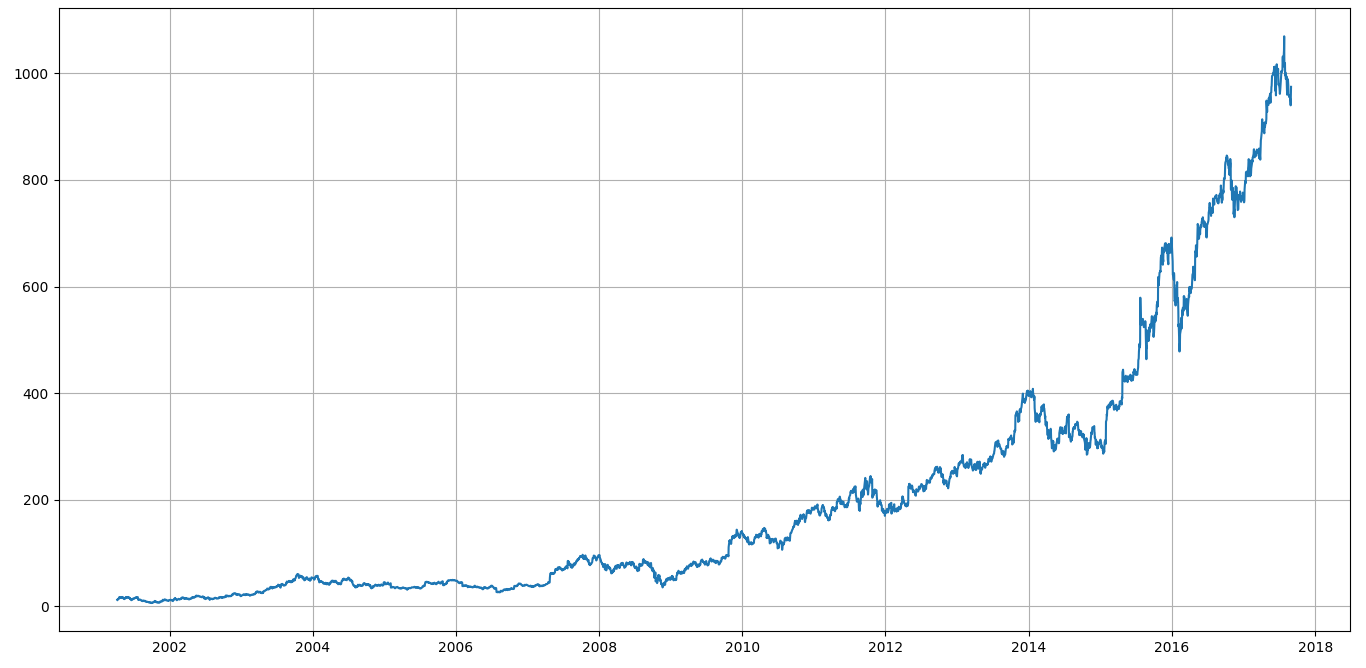
\includegraphics[width=1\textwidth, height=0.45\textwidth]{amazon_serie_novo}}
	\caption{Valores de abertura das ações da Amazon}
	\fonte{Elaborado pelo autor}
	\label{lingua}
\end{grafico}

Em contrapartida, as ações da Apple Inc contam com seus valores mais constantes. No período coletado, seu valor de abertura apresentou um mínimo de 0,93 e um máximo de 163,80 USD. No Gráfico 3 é possível observar o comportamento desta série.

\begin{grafico}[h]
	\centering
	\fbox{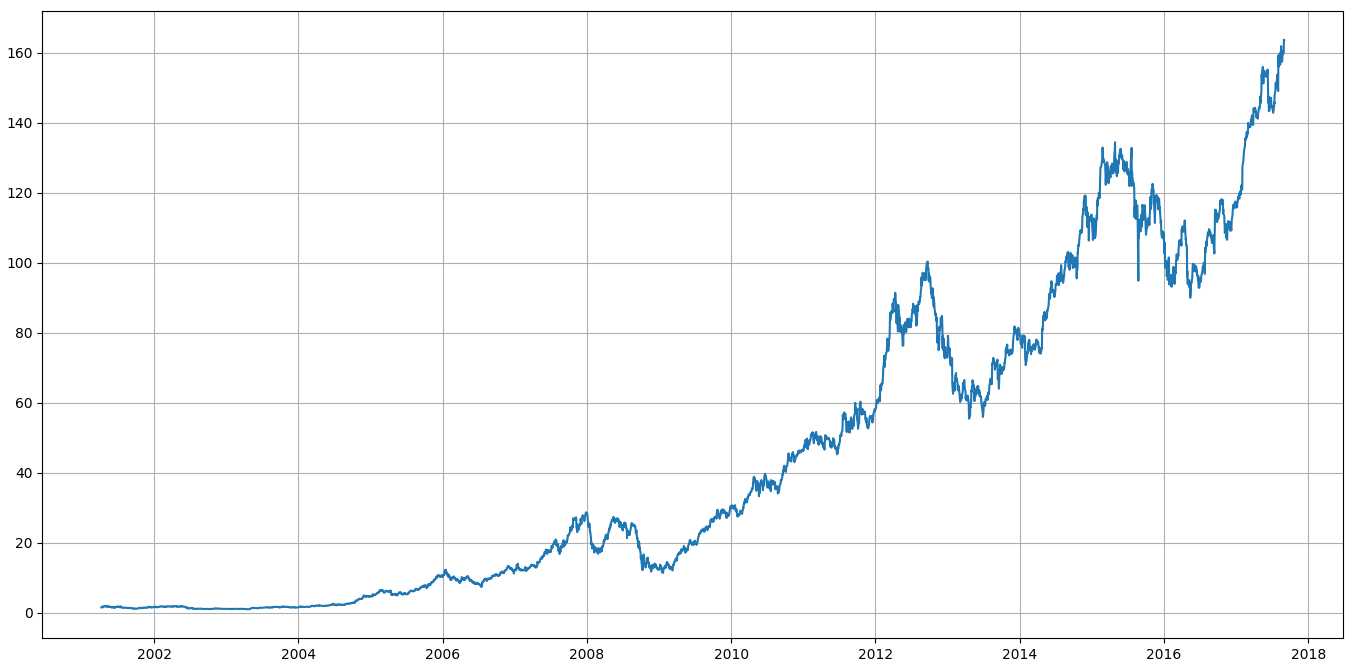
\includegraphics[width=1\textwidth, height=0.44\textwidth]{apple_serie_novo}}
	\caption{Valores de abertura das ações da Apple}
	\fonte{Elaborado pelo autor}
	\label{lingua}
\end{grafico}

Já as ações da Intel e Microsoft Corporation possuem os valores mais equilibrados dentre as empresas selecionadas para análise. Ao realizar a aquisição da série da Intel Corporation, pôde-se observar que a mesma trabalha com valores mais baixos e sem grande variação, principalmente se comparada a Amazon. No período coletado, seu valor de abertura apresentou um mínimo de 12,17 e um máximo de 38,25 USD. Por fim, a Microsoft Corporation também apresentou uma série bem equilibrada no período coletado, variando entre um valor de abertura mínimo de 15,20 e um máximo de 74,34 USD. Os Gráficos 4 e 5 demonstram, de forma mais intuitiva, as ações da Intel e Microsoft, respectivamente. 	

\begin{grafico}[h]
	\centering
	\fbox{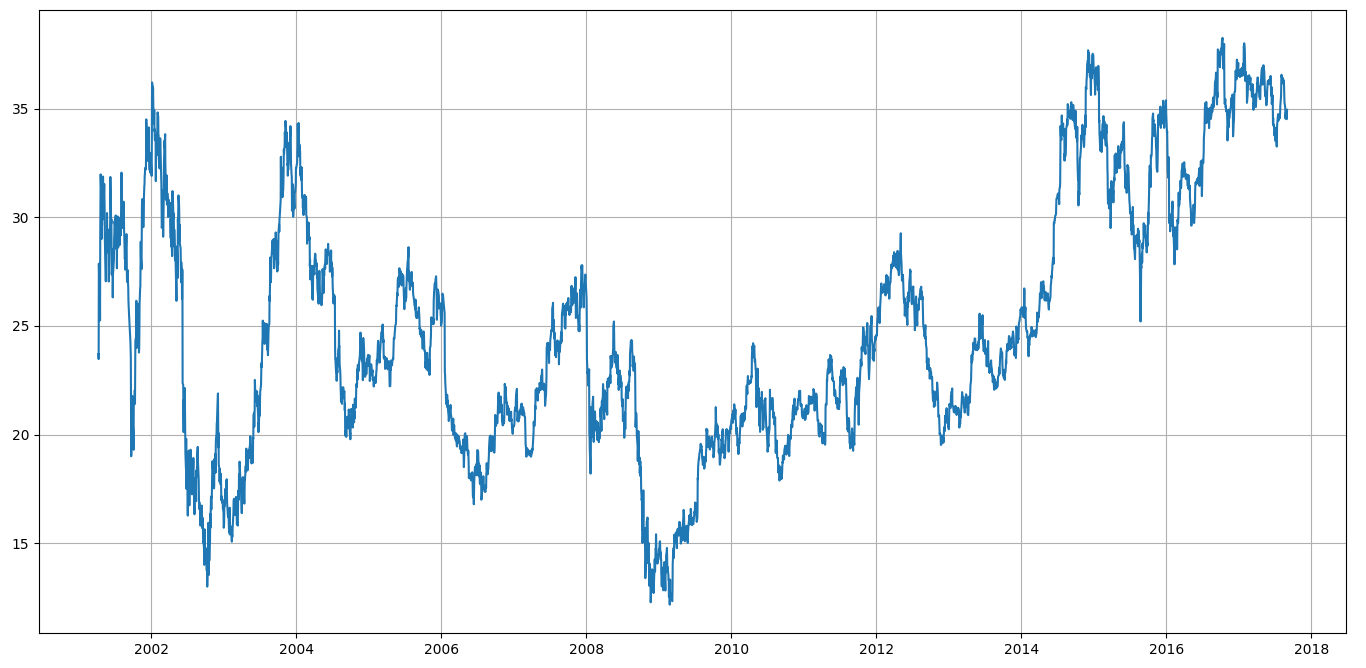
\includegraphics[width=1\textwidth, height=0.45\textwidth]{intel_serie_novo}}
	\caption{Valores de abertura das ações da Intel}
	\fonte{Elaborado pelo autor}
	\label{lingua}
\end{grafico}

\begin{grafico}[h]
	\centering
	\fbox{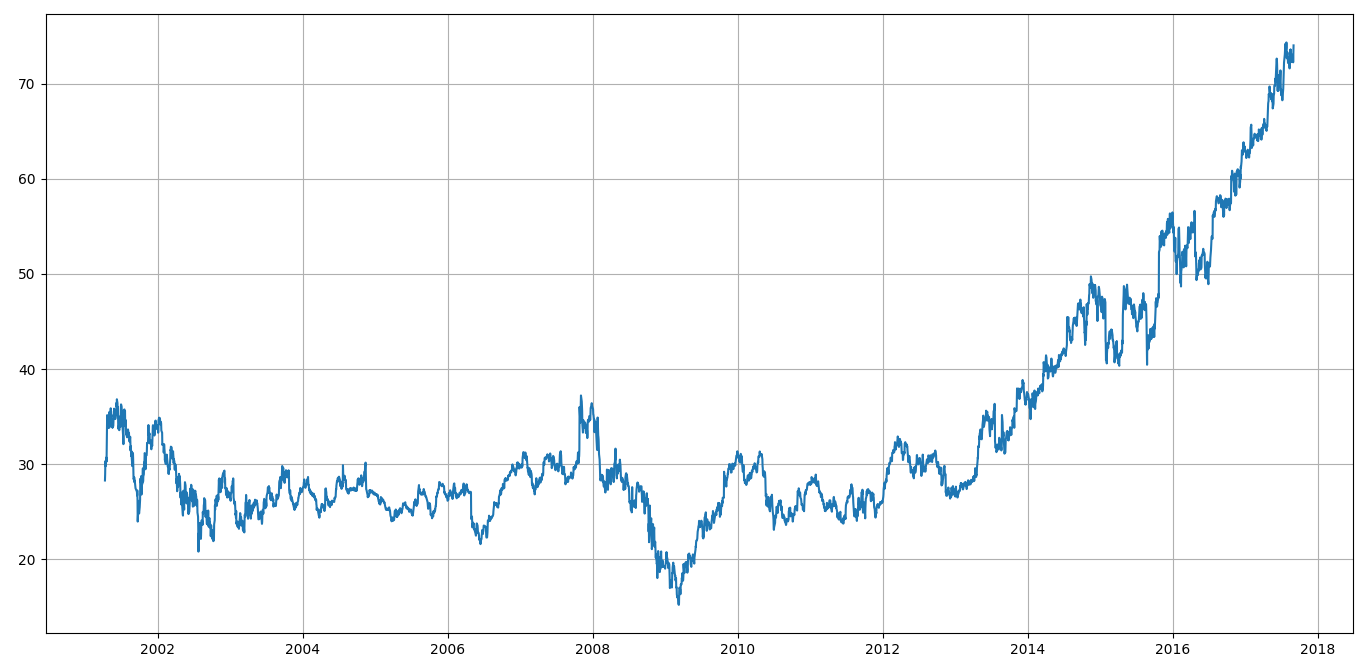
\includegraphics[width=1\textwidth, height=0.45\textwidth]{microsoft_serie_novo}}
	\caption{Valores de abertura das ações da Microsoft}
	\fonte{Elaborado pelo autor}
	\label{lingua}
\end{grafico}

Após evidenciar as características de todas as séries coletadas, pode-se concluir que as bases de dados são distintas, sendo de extrema importância para analisar a arquitetura da RNA.

\section{EXPLORANDO O \textit{DATAFRAME}}
O refinamento do modelo de dados coletado é de suma importância para agregar valor às informações do \textit{DataFrame} de cada empresa. Como especificado na Seção 4.3.1, faz-se necessário calcular alguns indicadores técnicos, que são consideradas informações expressivas que influenciam diretamente nos valores das ações.

Para desenvolver o cálculo das médias móveis de 10 e 26 dias, foi formada uma equação levando em consideração o exposto na Seção 4.3.1, o que proporciona de uma forma mais clara como realizar a implementação do algoritmo. A equação (5.1) demonstra este procedimento:
\begin{equation}\label{eq:MMS}
M_t = \dfrac{Z_t + Z_{t-1} + \dots + Z_{t-k+1}}{k},
\end{equation}
onde k é a quantidade de dias que se deseja calcular a média, t é o índice iterador da sequência que está sendo calculada e Z é o valor de fechamento da ação no momento t. A partir disto, foi desenvolvida uma função que realiza este cálculo. O Código 5 ilustra com detalhes esta implementação. 
\lstinputlisting[language=Python, label=cod-media-movel, caption=Implementação da função que realiza o cálculo da média móvel]{src/media-movel.py}

O Código 5 recebe como parâmetro o índice do \textit{DataFrame} e a quantidade de dias que se deseja calcular a média móvel. O algoritmo encontra este índice e, a partir disso, faz um incremento com o valor de fechamento. Após atingir o limite de incrementos necessários, levando em consideração a quantidade de dias, realiza a divisão e salva o valor em uma nova coluna do \textit{DataFrame}.

Já para o cálculo do indicador técnico MACD, o mesmo é realizado de forma mais simples com o auxílio da biblioteca pandas. O Código 6 cria uma nova coluna ao \textit{DataFrame} e realiza o cálculo da diferença, utilizando a função "sub", entre as duas médias móveis.
\lstinputlisting[language=Python, label=cod-media-movel, caption=Implementação da função que realiza o cálculo do MACD]{src/macd.py}

Finalizada a etapa de cálculo dos indicadores técnicos, todos os parâmetros necessários para iniciar a implementação da RNA, especificados no Capítulo 4, foram coletados e estruturados. A Figura 13 ilustra exatamente como ficou o \textit{DataFrame} após a inserção das novas colunas.
\begin{figure}[h]
	\centering
	\fbox{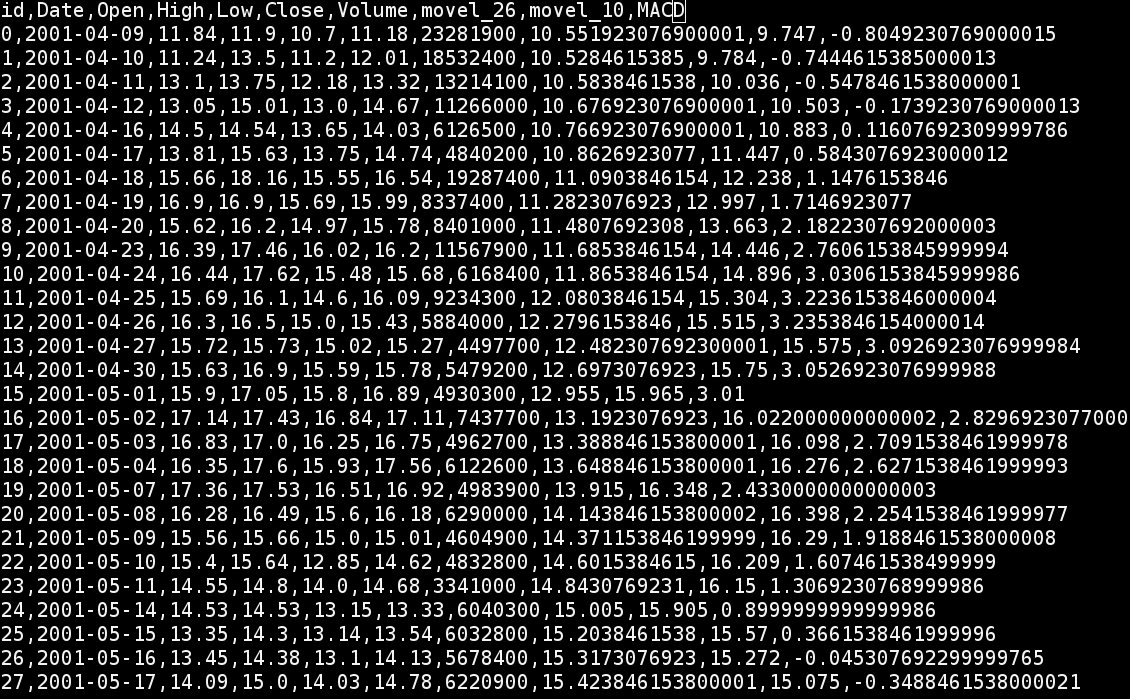
\includegraphics[width=0.8\textwidth, scale=0.5]{dados_formatados}}
	\caption{Exemplo do \textit{DataFrame} com os dados atualizados}
	\fonte{Elaborado pelo autor}
	\label{exec-dados-formatados}	
\end{figure}

\section{NORMALIZANDO OS DADOS}
Segundo \citeonline{Luiz}, o evento que antecede a etapa de treinamento de uma RNA é o processo de normalização dos dados de entrada e saída. Como o modelo proposto trabalha com a função de ativação sigmóide, detalhada na Seção 3.3.2, os dados devem ser normalizados entre um intervalo de [0,1]. A normalização consiste em adaptar uma base de dados com valores disintos, o que se aplica à realidade do presente trabalho, onde os valores das ações contam com intervalos de grande oscilação.

Considerando estas informações, duas equações foram especificadas para realizar a normalização e a desnormalização dos dados, com o objetivo de treinar a rede de forma mais eficaz, sendo elas:
\begin{equation}\label{eq:eq-normalizacao}
L_n = (L_o - L_{min}) / (L_{max} - L_{min})
\end{equation}
e
\begin{equation}\label{eq:eq-desnormalizacao}
L_o =  L_n * L_{max} + (1 - L_n) * L_{min},
\end{equation}
onde $L_o$ é o valor à ser normalizado, $L_n$ é o valor normalizado, $L_{min}$ e $L_{max}$ são os valores mínimos e máximos, respectivamente, dentre os valores da variável calculada.

A partir da equação (5.2), foi implementada uma função que normaliza uma determinada coluna de um \textit{DataFrame}. O Código 7 detalha o desenvolvimento do método.
\lstinputlisting[language=Python, label=cod-normalizador, caption=Implementação da função de normalização]{src/normalizador.py}

Para efetuar a desnormalização de um determinado valor, levando em consideração a equação (5.3), foi implementada uma função que realiza este procedimento, detalhada no Código 8.
\lstinputlisting[language=Python, label=cod-desnormalizador, caption=Implementação da função de desnormalização de um valor]{src/desnormalizador.py}  

Tendo em vista o desenvolvimento dos \textit{scripts} demonstrados, Código 7 e Código 8, foi utilizada a biblioteca matplotlib para gerar um gráfico e representar, com clareza, como ficaram os conjuntos de dados após o processo de normalização. O Código 9 detalha este procedimento.

\lstinputlisting[language=Python, label=cod-normalizado-grafico, caption=Classe que gera o gráfico dos dados normalizados]{src/normalizadorGrafico.py}

Após a execução do Código 9, foi renderizado o Gráfico 6 que demonstra os valores de cada empresa distribuidos entre o intervalo [0,1].

\begin{grafico}[h]
	\centering
	\fbox{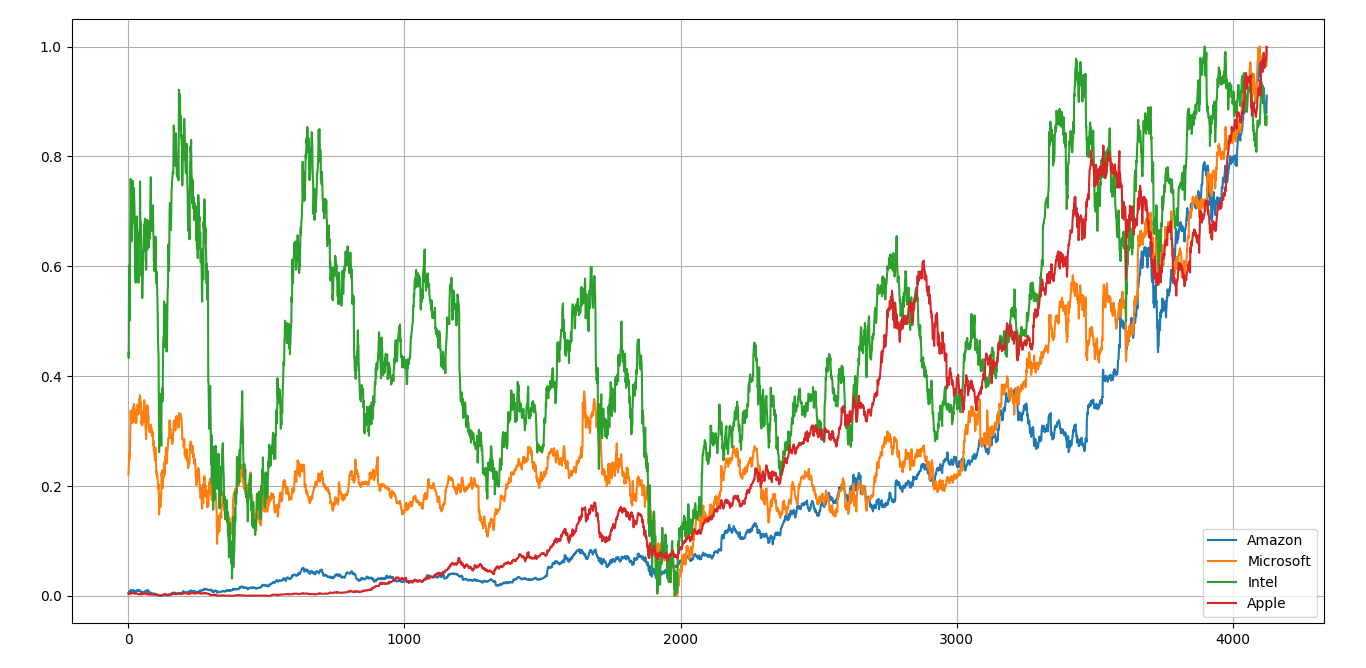
\includegraphics[width=1\textwidth]{normalizados_correto_banca}}
	\caption{Dados normalizados para treinamento}
	\fonte{Elaborado pelo autor}
	\label{lingua}
\end{grafico}

\section{DESENVOLVIMENTO DA REDE NEURAL ARTIFICIAL}
O ambiente de desenvolvimento do modelo de RNA proposto baseou-se nas ferramentas definidas no capítulo anterior, sendo elas a linguagem de programação Python, em sua versão 3.6.0, e a biblioteca PyBrain. Esta Seção detalha todos os procedimentos realizados para a implementação do modelo desenvolvido, evidenciando aspectos gerais de como trabalhar com Python e PyBrain.
\subsection{\textit{Script} para Criação de um Modelo \textit{FeedForward}}
A implementação de uma RNA com a topologia \textit{FeedForward} foi construída através do módulo pybrain.structure.networks. O mesmo tem como objetivo, especificar como são tratados o fluxo dos dados de entrada da rede. O Código 10 demonstra a importação do módulo e a criação da topologia determinada.

\lstinputlisting[language=Python, label=objeto-feedforward, caption=Construção de uma RNA com a estrutura \textit{FeedForward}]{src/FeedForward.py}

\subsection{Organização das Camadas do Modelo}
Após a implementação da topologia, faz-se necessário organizar suas camadas, assim como são tratados os respectivos neurônios das mesmas. Para a construção desta etapa, a biblioteca PyBrain oferece, através do módulo pybrain.structure, suporte à inserção via parâmetros, especificando a quantidade de variáveis para cada camada e, também, suas características. No Código 11 é possível observar a classe que implementa o método desenvolvido para a construção das camadas.

\lstinputlisting[language=Python, label=feedforward-layer, caption=Implementação da classe de criação de camadas]{src/feedforward_layers_pybrain.py}

Neste código são importados dois objetos do tipo \textit{Layer}, denominados \textit{LinearLayer} e \textit{SigmoidLayer}. A camada de entrada é composta pelo objeto \textit{LinearLayer}, onde os dados não sofrem nenhuma transformação, apenas transferindo-os para a camada posterior. A camada oculta é composta pelo objeto \textit{SigmoidLayer}, que implementa o cálculo da Equação (3.4) para os dados recebidos. Por fim, a camada oculta também é composta pelo objeto \textit{LinearLayer}, resultando na resposta da rede.   

Realizada a etapa de especificação das camadas e suas respectivas funcionalidades, é necessário adicioná-las, efetivamente, ao modelo de rede. Este procedimento deve ser feito por meio dos métodos \textit{addInputModule}, \textit{addModule} e \textit{addOutputModule}. O Código 12 demonstra a função desenvolvida para a inserção das camadas.

\lstinputlisting[language=Python, label=feedforward-layer, caption=Inserção de camadas em um modelo de RNA]{src/add_modulos.py}

Observando este código, pode-se notar que o mesmo recebe um modelo de rede como parâmetro, faz a inserção através dos respectivos métodos citados anteriormente e retorna a rede com a nova configuração.

A partir disto, a rede precisa identificar quais são as distribuições de conexões referente às camadas inseridas, para determinar o fluxo de trabalho dos dados. Este procedimento é realizado através do objeto \textit{FullConnection}, que determina a ligação entre as camadas. Como o modelo é composto por 3 camadas, realizou-se duas conexões, uma entre a camada de entrada e a camada oculta e outra entre a camada oculta e a camada de saída. No Código 13 é demonstrado o método desenvolvido para criar esta funcionalidade.

\lstinputlisting[language=Python, label=feedforward-connection, caption=Conectando as camadas criadas na RNA]{src/conexoes-camadas.py}

Concluída a fase de inserção das conexões, apresentada no Código 13, fez-se necessário inserir os pesos iniciais da rede. Este procedimento foi executado através do método \textit{sortModules}, disponbilizado pela biblioteca PyBrain, que adiciona, de forma aleatória, os pesos em um intervalo [-2,2].

\subsection{Treinamento da Rede}
Para o desenvolvimento do treinamento a biblioteca PyBrain utiliza dois módulos principais, sendo eles o pybrain.datasets, que é responsável por especificar qual o modelo de aprendizado que a rede trabalha, e, para o caso do aprendizado supervisionado, o módulo pybrain.supervised, que contém os respectivos algoritmos para a presente técnica.

Para mapear uma base de dados de aprendizagem supervisionada com as características desejadas, é necessário utilizar o método \textit{SupervisedDataSet}, onde o mesmo recebe como parâmetro a quantidade de entradas referente à base de dados utilizada e a quantidade de saídas desejadas. Para o presente trabalho, foi instanciada uma base de dados de treino para 8 entradas e 1 saída, seguindo as especificações da Seção 4.5.1.

Segundo \citeonline{haykin2000}, uma RNA, em média, utiliza até 1500 iterações para convergir. Tendo em vista esse valor, foi aplicado na rede um parâmetro de 200 iterações, buscando otimizar o tempo de treinamento, e de 1000 iterações, que se encontra dentro do limite desejável.

O Código 14 expõe o desenvolvimento do método que realiza a criação da base de treino.

\lstinputlisting[language=Python, label=base-treino-cod, caption=Construção de uma base de dados para treinamento]{src/base-treino.py}

Observando este código, pode-se notar que as linhas 2 e 3 são responsáveis por importar as dependências das bibliotecas utilizadas. Entre as linhas 5 e 9, é realizada a leitura do arquivo da empresa que foi transferida para a função via parâmetro (nome\_empresa). A linha 11 cria o objeto \textit{SupervisedDataSet} com suas devidas configurações, enquanto a linha 13 consome a base de treino a partir do \textit{DataFrame} sem seus oito últimos dias, que são utilizados para testes. Já a linha 14 inicia o processo de inserção das variáveis do \textit{DataFrame} para a nova base, através do método \textit{addSample}.

Também é possível notar, em relação ao \textit{DataFrame}, que são utilizados os dados normalizados para consumir a base de treinamento. Por fim, a distribuição da camada de saída, encontrada na linha 23, está sendo carregada pelo valor de abertura no dia posterior ao estudado, pelo índice [i + 1], caracterizando, de forma correta, a base de treino para o problema proposto.

Após concluído os procedimentos anteriores, pode-se iniciar, efetivamente, o treinamento da RNA. É importante ressaltar que, neste trabalho, o treino foi executado através do algoritmo \textit{Backpropagation}. O Código 15 demostra, de forma simples, como trabalhar com o algoritmo através da biblioteca PyBrain.

\lstinputlisting[language=Python, label=base-treino-cod, caption=Método de treinamento da RNA através do \textit{Backpropagation}]{src/realizaTreinamento.py}

A função implementada no Código 15, inicia o processo de treino a partir da chamada ao objeto \textit{BackPropTrainer}. Este, por sua vez, recebe alguns parâmetros no momento de sua criação, sendo eles: a rede neural em sí, a base de treinamento e a taxa de aprendizagem (\textit{learning rate}), detalhada na Seção 3.5.1. Segundo \citeonline{haykin2000}, um valor recomendado para o parâmetro \textit{learning rate} é de 0.4 (40\%). No presente trabalho, foi utilizada esta taxa como referência para o treinamento, evidenciada na linha 5 do Código 15. Já o parâmetro \textit{verbose}, auxilia o acompanhamento do erro quadrático médio durante o processo de treinamento, guardando as respectivas variações em um vetor unidimensional.

A partir disto, fez-se necessário realizar a chamada ao método \textit{train}. O mesmo recebe um valor responsável por limitar a quantidade de ciclos (iterações) na qual o modelo é treinado, através da variável \textit{epochs}.

O objeto \textit{NetworkWriter}, encontrado na linha 7, pertence ao pacote tools.customxml, implementando pela biblioteca, que utiliza uma classe que pode receber o estado atual de uma rede treinada e gravá-la em um arquivo \textit{eXtensible Markup Language} (XML). Segundo \citeonline{xml}, o XML foi criado para gerar linguagens de notação para necessidades especiais, de fácil manuseio e portabilidade de sua estrutura. Portanto, tendo em vista a capacidade de exportação da RNA para um arquivo XML, algumas possibilidades são oferecidas, tais como: retreinar a mesma, de forma simplificada, e testá-la quando desejado, sem a necessidade de realizar o processo de treinamento novamente.

A estrutura do arquivo gerado, levando em consideração a exportação realizada pelo Código 15, é demonstrada detalhadamente no Código 16.

\lstinputlisting[language=XML, label=base-treino-cod, caption=Estrutura do arquivo XML de uma RNA]{src/rede-feedforward-intel.xml}

Observando o Código 16, pode-se notar que todas as configurações executadas para construir a rede foram armazenadas dentro de suas respectivas características, denominadas \textit{tags}. As \textit{tags} foram padronizadas para que, no momento de leitura da RNA, através do objeto \textit{networkReader}, todo o ambiente seja importado de forma correta. Analisando as linhas 3, 6 e 14, por exemplo, é possível notar alguns dos parâmetros inseridos anteriormente na RNA. Além disso, também fica evidente a presença dos pesos sinápticos, entre a camada de entrada e a camada oculta, e, entre a camada oculta e a camada de saída, que são fundamentais para salvar um determinado estado da rede.

Por fim, tendo em vista o refinamento de todas as bases de dados coletadas e da implementação do modelo da RNA, todos os procedimentos necessários para realizar os testes foram desenvolvidos, com base na teoria e especificações dos capítulos anteriores. 
%% !TeX encoding = UTF-8

\chapter{ANÁLISE DOS RESULTADOS}\label{ch:resultados}
Este capítulo tem como finalidade apresentar os resultados obtidos através das implementações demonstradas no Capítulo 5.

\section{ANÁLISE DAS SÉRIES UTILIZADAS}
Após a implementação do modelo da RNA, através dos conjuntos de dados coletados, faz-se necessário avaliar como a respectiva técnica se comportou. Tendo isso em vista, a mesma foi aplicada em função do objetivo principal do trabalho, que é medir a capacidade de precisão de acerto no valor de abertura das ações. Portanto, foi elaborada, de forma independente, uma análise de eficácia do modelo para o cenário de cada empresa utilizada no presente trabalho. É importante ressaltar que os modelos foram implementados levando em consideração todos os \textit{scripts}, métodos e ferramentas utilizadas no capítulo anterior.

\subsection{Aplicação da rede na Intel Corporation}
A rede da Intel Corporation foi treinada com o objetivo de capturar o maior nível de variação possível dos dados, visando mapear um maior conjunto de padrões e, assim, responder de forma eficiente à dados dispersos através de uma boa capacidade de generalização. Tendo isso em vista, o período de treinamento preparado foi de 09/04/2001 até 21/08/2017, totalizando 4117 registros.

Para o presente caso foram construídos dois cenários de simulação, buscando obter um parâmetro de ciclos de treinamento adequado ao modelo de dados utilizado. As métricas definidas para análise, a partir destes ciclos de treinamento, são: o comportamento da função de custo que compõem o modelo (erro quadrático médio, EQM) e a margem de erro dos valores resultantes da rede, no período de 23/08/2017 a 31/08/2017, em relação aos valores reais. Os parâmetros utilizados foram: 200 e 1000 iterações.

\subsubsection{Treinamento com 200 Iterações}	
A ideia de executar o treinamento com uma quantidade baixa de iterações, é feita com o intuito de proporcionar um treinamento mais rápido e com resultados significativos, levando em consideração as características especificas do modelo de dados. Portanto, para quantificar como ocorreu o processo de treinamento, basta multiplicar o número de iterações (200) com o número de registros de testes (4117), resultando em um total de 823.400 exemplos calculados pela rede. O Gráfico 8 demonstra, de acordo com a quantidade de ciclos, a variação do EQM no primeiro cenário de teste com 200 iterações.
\begin{grafico}[h]
	\centering
	\fbox{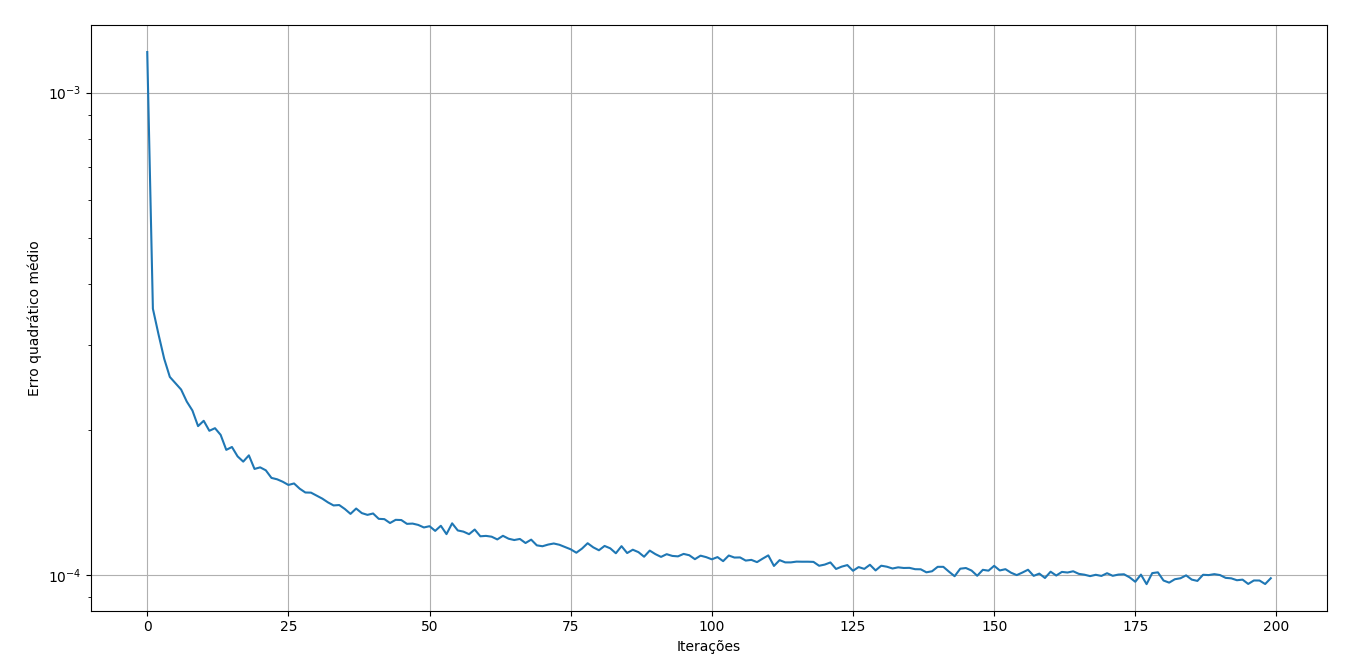
\includegraphics[width=1\textwidth]{erro_intel_primeiro}}
	\caption{Decaimento do EQM no treinamento da rede}
	\fonte{Elaborado pelo autor}
	\label{lingua}
\end{grafico}

O EQM de treinamento iniciou-se, na primeira iteração, com um erro percentual de 0.00248996652176 e, após o término das 200 épocas de treinamento, conclui-se com um erro percentual de 9.44359025338.$10^{-05}$. Analisando o gráfico, pode-se observar que os valores tiveram um decaimento constante até a iteração de número 125, enquanto que, nas 75 iterações posteriores, manteve os valores dos erros aproximados. A queda constante nas iterações iniciais está diretamente ligada a capacidade de aprendizado e adaptação ao modelo de dados.

Tendo em vista a variação dos erros obtidos após a primeira inicialização da rede, foi julgado necessário repetir o mesmo procedimento, visando observar o funcionamento do algoritmo de inicialização dos pesos e validar sua variação aplicada ao mesmo modelo de dados. Portanto, mais dois cenários foram executados com este objetivo. No segundo cenário, o erro foi iniciado com um percentual de 0.00102981131422 e, após o término das 200 épocas de treinamento, concluí-se com um percentual de 9.1790170623.$10^{-05}$. No terceiro cenário, o erro foi iniciado com um percentual de 0.00026991101482 e, após o término das 200 épocas de treinamento, concluí-se com um percentual de 9.49959768553.$10^{-05}$.

Analisando os três cenários, pode-se observar que apesar da rede ser iniciada com os pesos aleatoriamente, o EQM seguiu a mesma tendência para todos os casos, isso implica em uma confiabilidade maior por parte do algoritmo, pois o mesmo garante que novas inicializações, aplicadas ao mesmo modelo de dados, não resultam em valores muito distintos. Esta validação do algoritmo tem grande importância, pois com ela chega-se a definição de que os pesos iniciais da rede não precisarão, necessariamente, serem ajustados manualmente para encontrar um melhor resultado, pois aplicado ao mesmo modelo de dados, os erros seguem o mesmo padrão.

Após a análise do comportamento do EQM e a validação do algortimo de inicialização, os testes foram iniciados com o objetivo de verificar a precisão do modelo. Na Tabela 1 são detalhados os valores do período predito.
\begin{table}[h]
\centering
\caption{Período dos dados utilizados para testes: Intel Corporation}
\vspace{0.5cm}
\begin{tabular}{>{\centering\arraybackslash}m{2cm} >{\centering\arraybackslash}m{2cm} >{\centering\arraybackslash}m{2cm} >{\centering\arraybackslash}m{2cm} >{\centering\arraybackslash}m{2cm} >{\centering\arraybackslash}m{2cm}}
\toprule
Data    & Abertura   & Alta   & Baixa   & Fechamento   & Volume\\
\midrule
23/08/2017 & 34.54 & 34.81 & 34.38 & 34.66 & 196.481,34\\
24/08/2017 & 34.70 & 34.89 & 34.55 & 34.71 & 143.018,92\\
25/08/2017 & 34.82 & 34.93 & 34.58 & 34.67 & 147.268,29\\
28/08/2017 & 34.78 & 34.80 & 34.59 & 34.65 & 207.128,76\\
29/08/2017 & 34.51 & 34.75 & 34.46 & 34.73 & 158.436,68\\
30/08/2017 & 34.75 & 34.96 & 34.63 & 34.89 & 185.650,07\\
31/08/2017 & 34.94 & 35.18 & 34.87 & 35.07 & 163.667,72\\
\bottomrule
\end{tabular}
\end{table}

Os dados demonstrados na Tabela 1 foram refinados e normalizados de acordo com os métodos implementados no Capítulo 5. Após a execução deste processo, os mesmos foram inseridos na RNA para ativação. Posteriormente, foi realizada a desnormalização e os resultados apresentados. A Tabela 2 ilustra os resultados obtidos.
\begin{table}[h]
\centering
\caption{Resultados da predição realizada nos dados utilizados pela rede}
\vspace{0.5cm}
\begin{tabular}{>{\centering\arraybackslash}m{2cm} >{\centering\arraybackslash}m{2cm} >{\centering\arraybackslash}m{2cm} >{\centering\arraybackslash}m{2cm} >{\centering\arraybackslash}m{2cm}}
\toprule
Data    & Valor real   & Resultado    & Erro (\%) & Variação\\
\midrule
23/08/2017 & 34.54 & 34.73 & 0.550 & -0.19\\
24/08/2017 & 34.70 & 34.71 & 0.028 & -0.01\\
25/08/2017 & 34.82 & 34.79 & 0.086 & 0.03\\
28/08/2017 & 34.78 & 34.77 & 0.028 & 0.01\\
29/08/2017 & 34.51 & 34.75 & 0.695 & -0.24\\
30/08/2017 & 34.75 & 34.82 & 0.201 & -0.07\\
31/08/2017 & 34.94 & 34.99 & 0.143 & 0.05\\
\bottomrule
\end{tabular}
\end{table}

Analisando a Tabela 2, pode-se observar que os resultados obtidos foram significativos, onde o percentual de erro calculado, através do erro relativo percentual, não ultrapassou a margem 0.70\%, se aproximando, consideravelmente, dos valores reais. O erro médio, analisado para todo o período de predição, ficou em torno de 0.24\%, o que pode ser considerado baixo levando-se em conta o número de iterações utilizadas para treinar a RNA. Já a medida de dispersão dos erros em torno da média obtida (desvio padrão) foi de aproximadamente 0.26\%. Entretanto, analisando de forma mais detalhada cada valor resultante, pode-se evidenciar dois erros mais altos nos dias 23/08/2017 e 29/08/2017, com 0.550\% e 0.695\%, respectivamente. Tendo em vista que os valores mais próximos aos verdadeiros oscilaram no intervalo entre [34.70, 34.82], fica evidente que o modelo obteve erros mais altos em momentos de queda no valor desta série. A ocorrência destes erros acontece através da tendência de padrões em que a rede foi treinada, de forma crescente, não acompanhando assim as quedas bruscas no período. Isto fica mais claro observando o valor predito do dia 31/08/2017, onde o valor real obteve uma alta considerável, se comparada aos valores anteriores, porém não afetou a capacidade de precisão da RNA, mantendo a margem de erro pequena. O Gráfico 9 representa, de maneira ilustrativa, os resultados da série.
\begin{grafico}[h]
	\centering
	\fbox{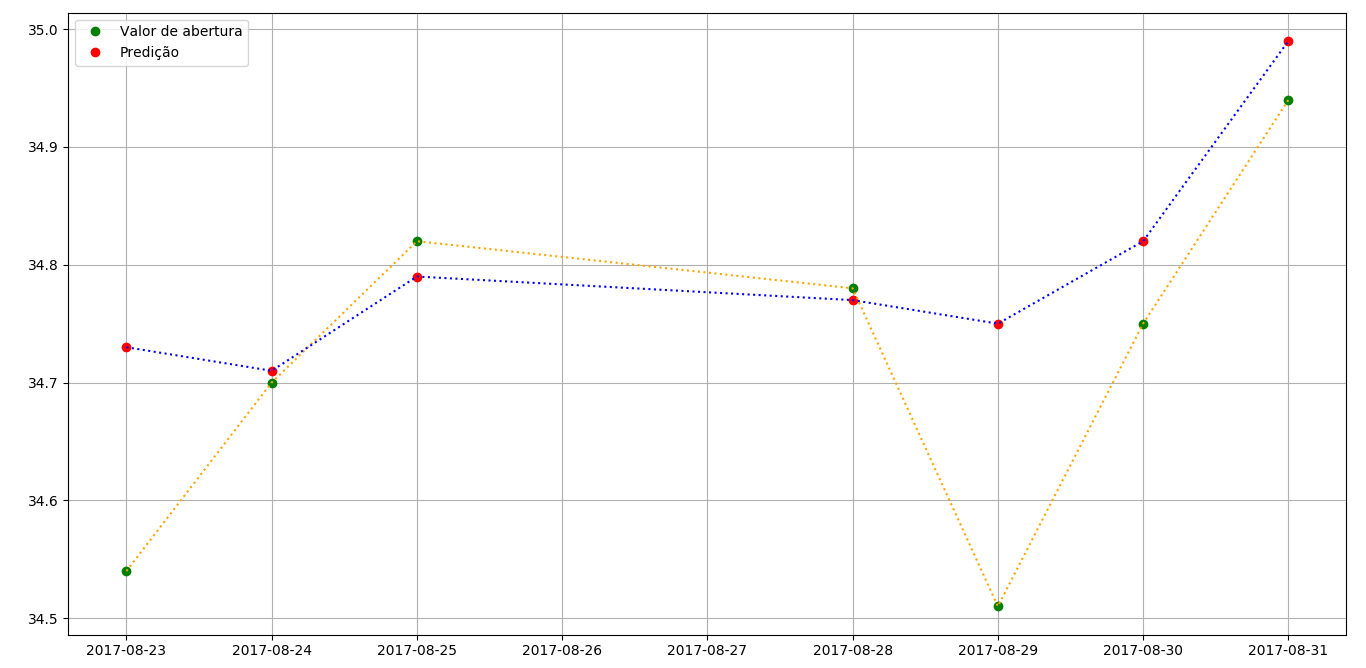
\includegraphics[width=1\textwidth]{predicao_intel}}
	\caption{Distribuição dos dados resultantes da RNA e seus valores esperados}
	\fonte{Elaborado pelo autor}
	\label{lingua}
\end{grafico}

Analisando o gráfico é possível observar como os resultados são próximos aos esperados. Os valores de abertura, nos respectivos dias testados, são representados por um ponto verde. Já os resultados obtidos pela rede são caracterizados pelo ponto vermelho. No Gráfico também fica evidente, de maneira ilustrativa, como a série não acompanhou as quedas do período e seguiu uma tendência crescente. 

\subsubsection{Treinamento com 1000 Iterações}	
Com a finalidade de comparar com a simulação anterior, foi realizado um teste com 1000 épocas de treinamento visando alcançar um resultado mais preciso e, também, para validar se o aumento na quantidade de iterações, no processo de treinamento, melhoram os resultados retornados pela rede.

Para quantificar como ocorreu o processo de treinamento, basta multiplicar o número de iterações (1000) com o número de registros de testes (4117), resultando em um total de 4.117.000 exemplos calculados pela rede.

Para o primeiro cenário a rede iniciou-se, na primeira iteração, com um erro percentual de 0.00664064049629 e, após o término das 1000 épocas de treinamento, conclui-se com um erro percentual de 8.7943563121853531.$10^{-05}$. Mais dois treinos distintos foram realizados visando encontrar alguma dispersão no erro obtido pela rede, como feito na análise anterior. Portanto, o segundo treino obteve um erro inicial de 0.00260377914122 e, após o término das 1000 épocas de treinamento, conclui-se com um percentual de 8.91402403614.$10^{-05}$. O terceiro treino obteve um erro inicial de 0.00496238079711 e, após o término das 1000 épocas de treinamento, o EQM do treinamento conclui-se com um percentual de 8.90814371631.$10^{-05}$.

Após a execução desses cenários de treinamento, pode-se concluir que a rede se comportou de forma estável em relação a quantidade de iterações, não distinguindo, de forma relevante, os valores dos pesos em diversas inicializações aleatórias. O Gráfico 10 representa, de maneira ilustrativa, o comportamento do EQM da rede treinada pelo primeiro cenário.
\begin{grafico}[h]
	\centering
	\fbox{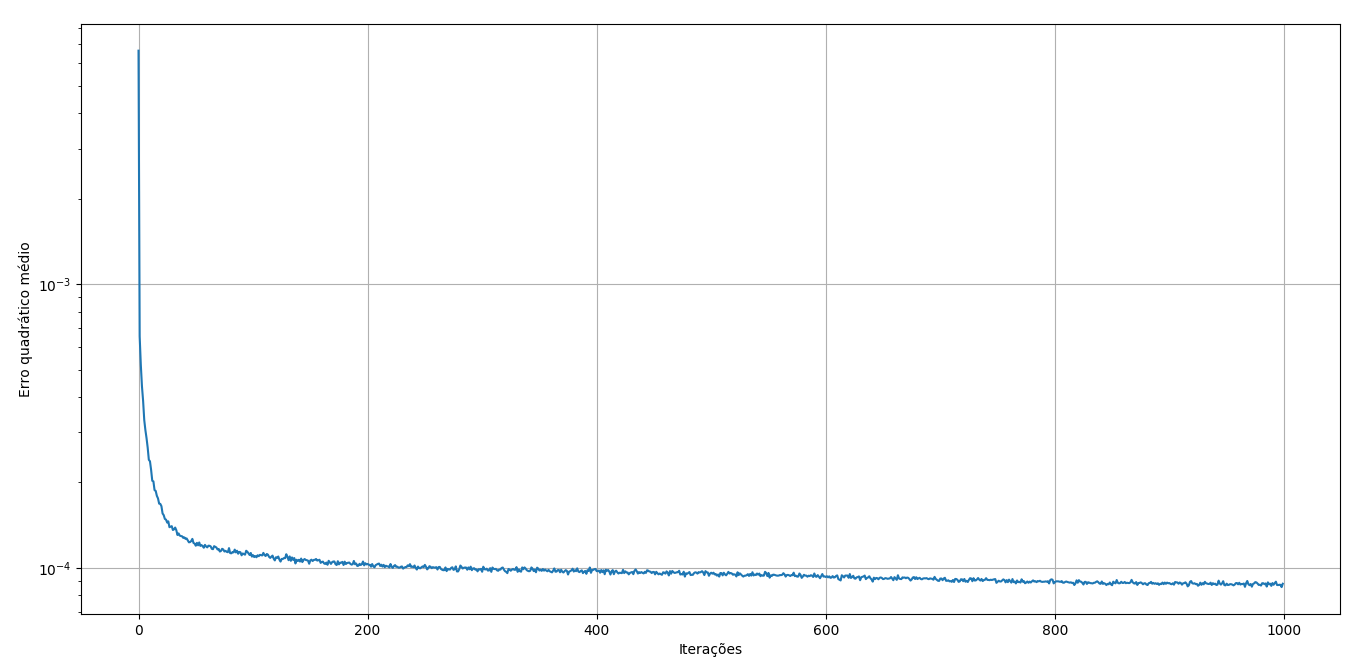
\includegraphics[width=1\textwidth]{erro_intel_1000iteracoes}}
	\caption{Decaimento do EQM no treinamento da rede}
	\fonte{Elaborado pelo autor}
	\label{lingua}
\end{grafico}

Analisando o Gráfico 10, pode-se observar que o erro obteve uma queda constante até 200 iterações, enquanto que, entre as iterações de número 200 até a de número 400, manteve o padrão com valores aproximados. Os últimos 600 ciclos mantiveram um decaimento mínimo do EQM.

Tendo em vista a simulação anterior, com 200 iterações, fica claro que a queda brusca e rápida aconteceria nas primeiras iterações, pois a base de dados utilizada é a mesma. Também é possível observar, através de um número maior de iterações, que o EQM obteve resultados mais baixos em comparação ao treino anterior.

O período aplicado para a realização dos testes foi o mesmo utilizado da Tabela 1. Os dados foram devidamente refinados, normalizados e, a partir disto, foram ativados na rede. Os resultados preditos, a partir da execução dos testes, são demonstrados na Tabela 3.
\begin{table}[h]
\centering
\caption{Resultados da predição realizada nos dados utilizados pela rede}
\vspace{0.5cm}
\begin{tabular}{>{\centering\arraybackslash}m{2cm} >{\centering\arraybackslash}m{2cm} >{\centering\arraybackslash}m{2cm} >{\centering\arraybackslash}m{2cm} >{\centering\arraybackslash}m{2cm}}
\toprule
Data    & Valor real   & Resultado    & Erro (\%) & Variação\\
\midrule
23/08/2017 & 34.54 & 34.67 & 0.376 & -0.13\\
24/08/2017 & 34.70 & 34.64 & 0.172 & 0.06\\
25/08/2017 & 34.82 & 34.71 & 0.315 & 0.11\\
28/08/2017 & 34.78 & 34.68 & 0.287 & 0.10\\
29/08/2017 & 34.51 & 34.65 & 0.405 & -0.14\\
30/08/2017 & 34.75 & 34.70 & 0.143 & 0.05\\
31/08/2017 & 34.94 & 34.84 & 0.286 & 0.10\\
\bottomrule
\end{tabular}
\end{table}

Analisando a Tabela 3, pode-se observar que os resultados obtidos foram significativos, onde o percentual de erro calculado, através do erro relativo percentual, não ultrapassou a margem 0.50\%, se aproximando consideravelmente dos valores reais. Porém, a média de todo o período analisado obteve um erro de 0.28\%, superior ao treinamento anterior. Já a medida de dispersão dos erros em torno da média obtida (desvio padrão) foi de aproximadamente 0.09\%. Sendo assim, pode-se concluir que o desvio padrão foi menor que o do primeiro cenário, devido ao fato dos erros mais altos (23/08/2017 e 29/08/2017) serem mais suaves. O Gráfico 11 representa, de maneira ilustrativa, os resultados da rede.

\begin{grafico}[h]
	\centering
	\fbox{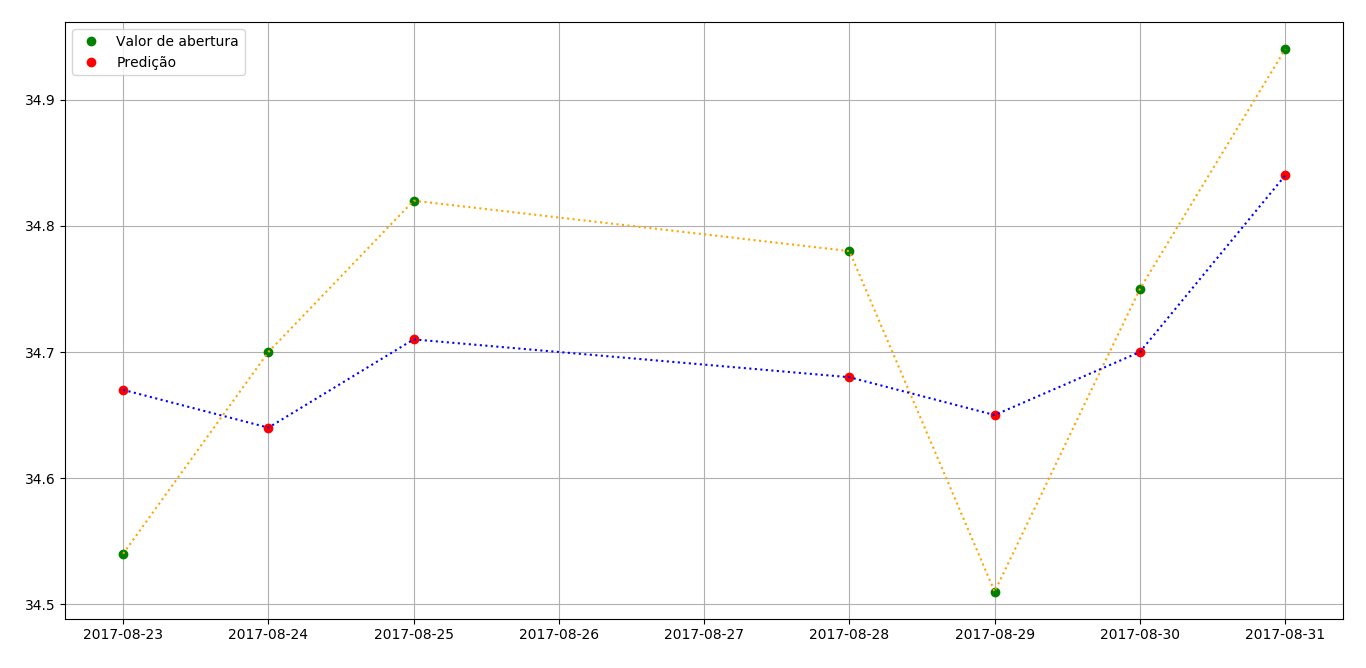
\includegraphics[width=1\textwidth]{predicao_intel_1000}}
	\caption{Distribuição dos dados resultantes da RNA e seus valores esperados}
	\fonte{Elaborado pelo autor}
	\label{lingua}
\end{grafico}

Apesar da diferença do erro percentual relativo entre os dois cenários ser de apenas 4\%, foi encontrada uma melhor parâmetrização para o presente modelo de dados utilizando um treinamento com 200 iterações, pois a exatidão dos valores preditos foram mais eficazes neste método de treinamento. Sendo assim, chega-se a definição que nem sempre um número maior de ciclos de treinamento aumentam a precisão da RNA. Neste caso, a rede sofreu uma convergência do EQM em torno de 200 iteraçoes, este detalhe pode ser observado visualizando o comportamento do Gráfico 10. Dessa forma, as iterações posteriores propagaram o erro de forma desnecessária, alterando assim os pesos sinápticos dos neurônios e, automaticamente, causando uma maior dispersão nos resultados. Este processo ocorrido na segunda simulação, na literatura, é denominado \textit{Overtraining}, detalhado no Capítulo 3.

\subsection{Aplicação da rede na Microsoft Corporation}
A rede da Microsoft Corporation foi treinada utilizando as mesmas técnicas da Intel Corporation, ou seja, com o intuito de capturar o maior nível de variação possível dos dados, visando mapear um maior conjunto de padrões e, assim, obter uma boa capacidade de generalização. Tendo isso em vista, o período de treinamento preparado foi de 09/04/2001 até 21/08/2017, totalizando 4117 registros.

Para o presente caso foram construídos dois cenários de simulação, buscando obter um parâmetro de ciclos de treinamento adequado ao modelo de dados utilizado. As métricas definidas para análise, a partir destes ciclos de treinamento, são: o comportamento da função de custo que compõem o modelo (erro quadrático médio, EQM) e a margem de erro dos valores resultantes da rede, no período de 23/08/2017 a 31/08/2017, em relação aos valores reais. Os parâmetros de ciclos de treinamento utilizados foram: 200 e 1000 iterações.

\subsubsection{Treinamento com 200 Iterações}	
O treinamento com 200 iterações foi executado com o objetivo de verificar a capacidade de precisão da rede com um número menor de iterações. Para quantificar como ocorreu o processo de treinamento, basta multiplicar o número de iterações (200) com o número de registros de testes (4117), resultando em um total de 823.400 exemplos calculados pela rede.

Para este caso, a RNA foi inicializada duas vezes com o objetivo de observar o comportamento e a tendência do EQM em relação ao algoritmo de inicialização. No primeiro cenário, a rede iniciou-se com o EQM em 0.0018579672451418453 e, após as 200 iterações, conclui-se com um erro de 3.6623220378015219.$10^{-05}$. No segundo cenário, o erro foi inicializado com 0.0047598765727053707 e, após as 200 iterações, conclui-se com um erro de 3.8483854181673219.$10^{-05}$.

É possível verificar, através dos dois cenários executados, que o erro seguiu a mesma tendência para os dois casos, com um erro final próximo a 3.$10^{-05}$. Tendo isso em vista, possíveis inicializações distintas aplicada ao modelo de dados da Microsoft Corporation não irão resultar em valores muito distintos, pois a diferença do erro é mínima.

Para demonstrar, de maneira mais clara, o comportamento do erro obtido pela rede em todo processo de treinamento, o Gráfico 12 demonstra, de acordo com a quantidade ciclos, a variação do EQM no primeiro cenário de teste.
\begin{grafico}[h]
	\centering
	\fbox{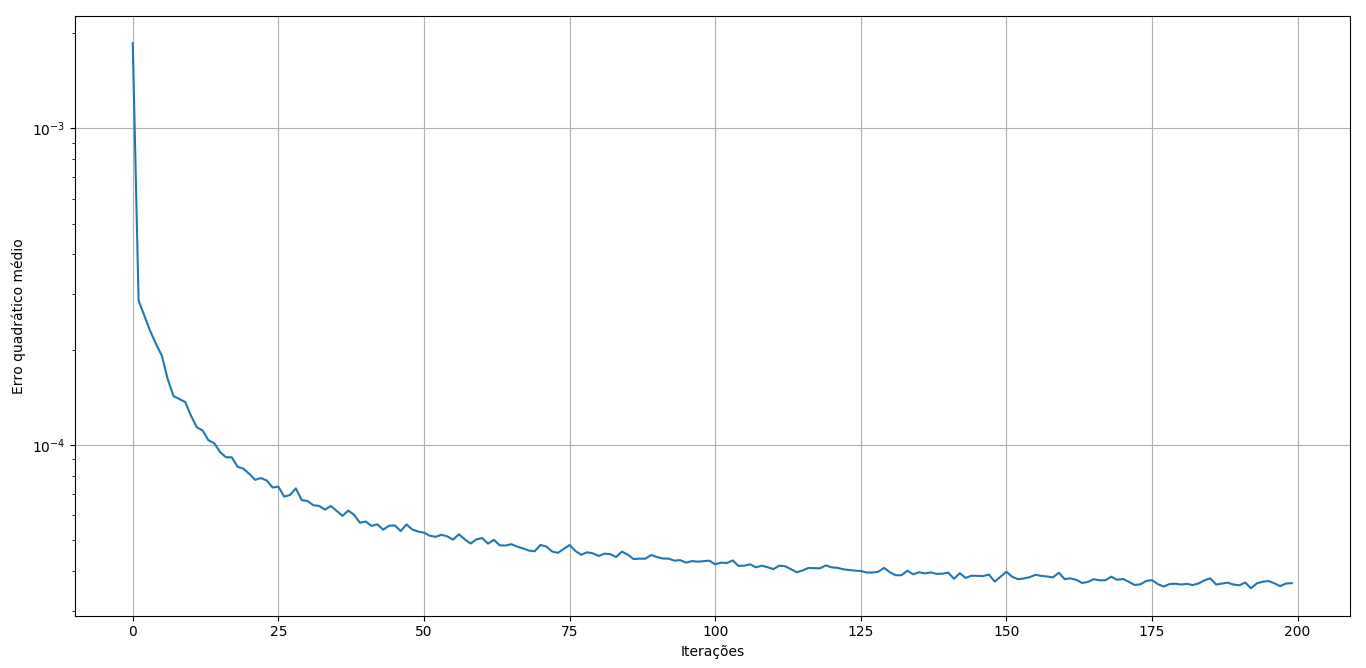
\includegraphics[width=1\textwidth]{erro_microsoft_200_segundo_cenario}}
	\caption{Decaimento do EQM no treinamento da rede}
	\fonte{Elaborado pelo autor}
	\label{lingua}
\end{grafico}

Analisando o gráfico, pode-se observar que os valores tiveram um decaimento constante até a iteração de número 125, enquanto que, nas 75 iterações posteriores, manteve os valores dos erros aproximados. A queda constante nas iterações iniciais está diretamente ligada a capacidade de aprendizado e adaptação ao modelo de dados.

Após a análise do comportamento do EQM e a validação do algortimo de inicialização, os testes foram iniciados com o objetivo de verificar a precisão do modelo. Na Tabela 4 são detalhados os valores do período predito.
\begin{table}[h]
\centering
\caption{Período dos dados utilizados para testes: Microsoft Corporation}
\vspace{0.5cm}
\begin{tabular}{>{\centering\arraybackslash}m{2cm} >{\centering\arraybackslash}m{2cm} >{\centering\arraybackslash}m{2cm} >{\centering\arraybackslash}m{2cm} >{\centering\arraybackslash}m{2cm} >{\centering\arraybackslash}m{2cm}}
\toprule
Data    & Abertura   & Alta   & Baixa   & Fechamento   & Volume\\
\midrule
23/08/2017 & 72.96 & 73.15 & 72.53 & 72.72 & 137.665,07\\
24/08/2017 & 72.74 & 72.86 & 72.07 & 72.69 & 170.982,82\\
25/08/2017 & 72.86 & 73.35 & 72.48 & 72.82 & 127.943,01\\
28/08/2017 & 73.06 & 73.09 & 72.55 & 72.83 & 145.697,15\\
29/08/2017 & 72.25 & 73.16 & 72.05 & 73.05 & 114.783,82\\
30/08/2017 & 73.01 & 74.21 & 72.83 & 74.01 & 168.978,01\\
31/08/2017 & 74.03 & 74.96 & 73.80 & 74.77 & 276.528,11\\
\bottomrule
\end{tabular}
\end{table}

Os dados demonstrados na Tabela 4 foram refinados e normalizados de acordo com os métodos implementados no Capítulo 5. Após a execução deste processo, os mesmos foram inseridos na RNA para ativação. Posteriormente, foi realizada a desnormalização e os resultados apresentados. Na tabela 5 é possível verificar os resultados obtidos pela rede.

\begin{table}[h]
\centering
\caption{Resultados da predição realizada nos dados utilizados pela rede}
\vspace{0.5cm}
\begin{tabular}{>{\centering\arraybackslash}m{2cm} >{\centering\arraybackslash}m{2cm} >{\centering\arraybackslash}m{2cm} >{\centering\arraybackslash}m{2cm} >{\centering\arraybackslash}m{2cm}}
\toprule
Data    & Valor real   & Resultado    & Erro (\%) & Variação\\
\midrule
23/08/2017 & 72.96 & 72.94 & 0.027 & 0.02\\
24/08/2017 & 72.74 & 72.61 & 0.028 & 0.13\\
25/08/2017 & 72.86 & 72.50 & 0.086 & 0.36\\
28/08/2017 & 73.06 & 72.73 & 0.028 & -0.33\\
29/08/2017 & 72.25 & 72.64 & 0.695 & -0.39\\
30/08/2017 & 73.01 & 72.82 & 0.201 & 0.19\\
31/08/2017 & 74.03 & 73.75 & 0.143 & 0.28\\
\bottomrule
\end{tabular}
\end{table}

Analisando a Tabela 5, pode-se observar que os resultados obtidos foram significativos, onde o percentual de erro calculado, através do erro relativo percentual, não ultrapassou a margem 0.70\%, se aproximando, consideravelmente, dos valores reais. O erro médio, analisado para todo o período de predição, ficou em torno de 0.17\%, o que pode ser considerado baixo levando-se em conta o número de iterações utilizadas para treinar a RNA. Já a medida de dispersão dos erros em torno da média obtida (desvio padrão) foi de aproximadamente 0.23\%.
%% !TeX encoding = UTF-8

\chapter{CONCLUSÕES E SUGESTÕES PARA FUTUROS TRABALHOS}\label{ch:conclusao}
\section{CONCLUSÕES} 
O uso das bibliotecas que Python oferece para a mineração de dados...

- Resgatar o objetivo

- Comentar as ferramentas estudadas

- Comentar as ferramentas utilizadas

- Breve resumo dos resultados

- Pontos positivos e negativos (O fato de não ter o perfil real)


\section{SUGESTÕES PARA FUTUROS TRABALHOS}

%
%7.2
%Pensar em outra API (Aplicação para previsão de resultados) ou rede social, baseando-se numa pergunta específica

%\bookmarksetup{startatroot}

%==============================================================================
% ELEMENTOS PÓS-TEXTUAIS
%==============================================================================
\postextual

% ------------------------------------ %
% Arquivo de bibliografias do trabalho %
% ------------------------------------ %
\label{biblio}\bibliography{Configuracoes/referencias}

{\ }\label{fimBiblio}

\pagebreak
\ 


%==============================================================================
% APÊNDICES
%==============================================================================

%\begin{apendicesenv}% Apêndices: inserir se necessário
%\partapendices
%  \input{Extras/apendice1}
%  \input{Extras/apendice2}
%\end{apendicesenv}

%\begin{anexosenv}% Anexos: inserir se necessário
%\partanexos
% \input{Extras/anexo1}
% \input{Extras/anexo2}
% \input{Extras/anexo3}
%\end{anexosenv}

\printindex		% Indice Remissivo


\end{document}
